\documentclass[11pt,letterpaper]{article}

\usepackage{graphicx}
\usepackage{subfig}


\begin{document}

    \title{The effects of sequence learning on the correlated activity in the Hierarchical Temporal Memory}
	\author{Victor Hernandez-Urbina\\
	    \texttt{vhernandezurbina@numenta.com}
	}
	%\email[]{vhernandezurbina@numenta.com}
    \date{\today}
    
    \maketitle
    
    \begin{abstract}
        Correlated activity in groups of neurons has been reported
        in many studies and in different experimental protocols in practically all
        areas of neuroscience. Although its use has proven to be useful to reveal
        functional connectivity among different brain areas,
        its role in neural information processing is still under much debate.
        In the present study, we use a biologically plausible neural network model to
        investigate the nature of correlated activity in the context of 
        sequential learning.
        We are able to replicate some observations from experimental
        neuroscience, and to present some predictions regarding the effect
        of learning on the structure of neural correlations.
    \end{abstract}
    
    %\maketitle
    
    \section{Introduction}
        Correlated activity of population of neurons provides relevant information
        regarding the functional connectivity of brain networks.
        The observation of correlated activity is the first step towards revealing 
        a purported causal relationship between two different brain areas.
        For correlated activity to emerge in a single region, there has to be
        correlated activity within the region.
        The study of correlated activity at the level of single cells poses enormous
        experimental challenges particularly when trying to correlate the observed
        correlation patterns to the stimulus being presented to a sensory organ due to
        the noisy nature of neurons.
        
        Moreover, studying brain correlated activity imposes computational
        challenges as it requires the analysis of large amounts of data from
        simultaneously recorded neurons.
        This is the main reason why most studies of correlations at the level
        of individual neurons are primarily focused on pairwise cell activity.
        
        The correlated activity within a group of neurons might provide some
        insights regarding the encoding mechanisms of the neural substrate.
        Information might be encoded both in the individual activity of neurons,
        as well as in the correlations among their 
        activities~\cite{eyherabide2013and}.
        Thus, the study of neural correlations is relevant not only to reveal
        functional connectivity in the brain without recurring to invasive
        methods but also to decipher the neural code.

        Neural correlations have been measured in many cortical regions in
        different experimental conditions over the past two decades.
        Observations vary across studies.
        However, most of them agree that pairwise correlations are typically
        small and positive.
        Nevertheless, small and perhaps undetectable correlation in pairs of
        neurons can have a large effect at the population level~\cite{averbeck2006neural}.
        That is, even if we observe low correlated activity when considering
        the spiking activity of only two cells, the network might
        actually exhibit highly correlated states in the form of
        synchronous activation or quiescence of groups of neurons which
        carry vital information to the system.

        Cohen and Kohn present a summary of relevant
        studies regarding neuronal correlations in different brain areas, and under
        different behavioural settings~\cite{cohen2011measuring}.
        These authors describe some experimental factors that contribute to
        the variability in observed measurements.
        These include measurements performed on few spikes per trial, and 
        the length of the time window in which spikes are counted, among others.
        Such factors might lead to incorrect interpretations of the correlated,
        or decorrelated activity, of neuronal populations.
        
        It has been observed that correlations are usually higher for neuron pairs 
        that are closer to each other, and also possess similar tuning properties
        As well, it has been reported without a satisfactory explanation that neural correlations
        are weak in the input layers of primary sensory cortex, and that
        correlations in motor areas seem to be consistently lower than those
        in sensory cortex.
        
        As mentioned above, most researchers agree that neural correlations between
        pairs of cells are low.
        Schneidmann and colleagues show in a study
        based on neuronal activity in the retina of salamanders exposed to natural
        video clips that weak pairwise correlations
        coexist with strong collective behaviour in the response of groups
        of neurons~\cite{schneidman2006weak}. 
		Figure \ref{fig1} shows the distribution of pairwise correlation coefficients
		obtained from such study.
        As well, these authors suggest that correlated neural activity
        provides a neural code with error-correcting properties.

 		\begin{figure}[t]
			\centering
			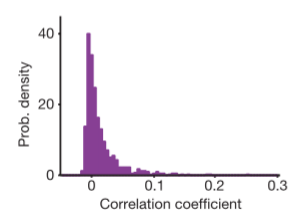
\includegraphics[scale=0.75]{Schneidman3.png}
			\caption{
			    Pairwise correlation coefficients obtained from
			    the activity of retinal ganglion cells of salamander.
			    Correlations between neuron pairs are weak.
			    (Image taken from Ref.~\cite{schneidman2006weak})
			}
			\label{fig1}
		\end{figure} 
		
        In their study, Schneidmann and colleagues estimate the probability of
        observing particular binary words which are obtained from raster
        plots of spike trains from retinal activity compared to the
        probability of observing such words in a random model based on Poisson
        spiking.
        This process is shown in Fig.~\ref{fig2}.
        A subsample comprising $10$ neurons from the spiking activity of 
        retinal ganglion cells is considered along with a time window
        $\Delta t$ in which the occurrence of action potentials is
        measured for all cells in the sample.
        This would yield binary patterns or words of length $10$,
        if for a given time $t$ the $i$-th cell fires, then a $1$ is
        placed in the $i$-th position of the binary pattern, and $0$
        otherwise.

		\begin{figure}[t]
			\centering
			\subfloat[Raster plot obtained from spike trains of $40$ retinal ganglion cells.]{%
				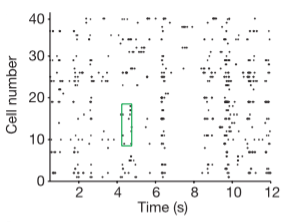
\includegraphics[scale=0.6]{Schneidman1.png}
				\label{fig1:a}
			}
			\subfloat[Generation of binary patterns from neural activity.]{%
				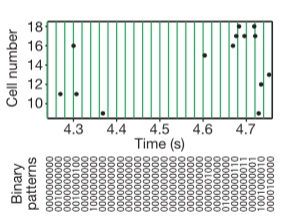
\includegraphics[scale=0.6]{Schneidman2.png}
				\label{fig1:b}
			}
			\caption{
			    Binary patterns from the activity of retinal ganglion cells are
			    obtained by subsampling the spike trains from $40$ cells
			    and considering a time window $\Delta t$ in which the occurrence
			    of action potentials is measured.
			    The green box in (\emph{a}) corresponds to the upper raster plot
			    in (\emph{b})
			    If cell $i$ emits a spike within $\Delta t$, a $1$ is placed
			    at the $i$-th position in the binary pattern, and $0$
			    otherwise.
			    In this example, the binary patterns consist of $10$ bits.
			    (Image taken from Ref.~\cite{schneidman2006weak})
			}
			\label{fig2}
		\end{figure}     
        
        The researchers reported that although the pairwise neural correlations
        are low, the probability of observing particular binary words is larger
        than predicted by the random model. Thus, implying that the collective
        behaviour of these cells exhibit strong correlated states.
        This is shown in Fig.~\ref{fig3}.
        The rate of occurrence for some binary patterns is larger than what is
        predicted by the independence assumption, that is, assuming that
        the firing of each cell is independent from one another.
        This implies that although the activity of neuron pairs is weakly
        correlated, the population exhibits states of activation that
        occur more often than predicted by chance.
        Such population states might encode information that is relevant
        to the system.
        As a corollary, this study also implies that it is not required to
        study higher-order correlations.
        Such results are also confirmed when fitting a maximum entropy
        model to their data~\cite{schneidman2006weak,schneidman2003network}.

 		\begin{figure}[t]
			\centering
			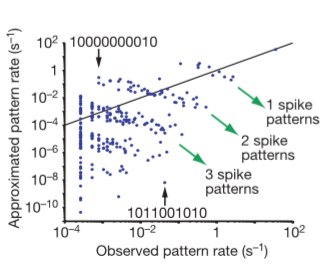
\includegraphics[scale=0.75]{Schneidman4.png}
			\caption{
			    Rate of occurrence of each pattern predicted if all
			    cells are independent (Poisson model) versus the observed
			    measured rate from retinal ganglion cells.
			    Black solid line shows equality.
			    Two examples of extreme misestimation of the predicted pattern
			    rate by the independent model vs. the observed rate are highlighted.
			    (Image taken from Ref.~\cite{schneidman2006weak})
			}
			\label{fig3}
		\end{figure} 
        
        What are the origins of correlated activity?
        Authors differ regarding the alleged origin of neural correlations.
        Some claim that it is the inevitable consequence of shared input in
        groups of neurons, while others have shown in models how shared input
        is not a necessary factor for correlations to 
        emerge~\cite{renart2010asynchronous,ecker2010decorrelated}.
        Moreover, it has been suggested that correlated activity might in
        fact be detrimental for neural processing as it reduces the
        accuracy of neural encoding~\cite{renart2010asynchronous}.
        
        However, Ecker and co-workers suggest that
        such is the case for homogeneous populations of neurons, in which
        all cells possess the same linear tuning properties~\cite{ecker2011effect}.
        In this scenario, reduced neural correlations induced by attention
        or by learning and adaptation have been interpreted as evidence
        for a more efficient population code.
        In their model, Ecker and colleagues show that increasing the amount
        of correlations can substantially improve encoding accuracy,
        when the neural population comprises heterogeneous tuning properties,
        a feature that is more akin to real brain networks.
        Such improvement results from a drop in noise entropy which is generally
        associated with increasing correlated activity.
        Thus, in contrast to current belief, these authors found that
        decreasing correlations does not necessarily lead to increased
        information.
        If correlations are large enough, increasing them can substantially
        increase the encoding accuracy~\cite{ecker2011effect}.
        
        One question that remains open is what is the role of neural correlations on learning? 
        Or better said, how the process
        of learning affects the quality of the structure of correlations?
        Researchers have found that the correlation structure is a target for
        learning-dependent enhancement of sensory encoding~\cite{jeanne2013associative}.
        The study focuses on the differences between the correlations in the tuning curves
        of two cells, and their correlated activity when presented with a fixed stimulus.
        The goal of the study is to reveal how these differences impact an organism's
        behaviour.
        The authors observed the behavioural responses of birds to particular stimulus motifs
        which can be thought of elemental auditory sequences.
        Authors claim that learning selectively alters the structure of correlations,
        both in the correlation between tuning curves, and in the correlated response
        of two different neurons for a particular stimulus.
        Such observation holds for stimuli that are behaviourally relevant
        Thus, this study concludes that the structure of correlations in a population of
        neurons carries biologically significant information that is independent of
        single neurons, and that is crucial to the transformation of purely sensory codes
        into neural signals that ultimately drive learned behaviour~\cite{jeanne2013associative}.
        
        Neural correlations are significantly smaller in trained versus naive animals, which is
        thought to result in an improvement on coding efficiency~\cite{gu2011perceptual} confirming
        the suggestions made by Ecker and colleagues~\cite{ecker2011effect}.
        In a study based on measuring the responses of neuron pairs in the dorsal medial superior
        temporal area (MST) of 
        awake monkeys subject to training, authors found that training reduced neural
        correlations uniformly regardless of the tuning similarity between pairs of neurons.
        Their study concludes that the impact of correlated activity on population coding depends
        on the structure of the neural noise and its dependence on the correlations between
        tuning curves.
        
        Other authors, however, have observed that learning actually increases the correlated
        activity in a population of neurons.
        In an experiment set in the context of Bayesian models of perception, Berkes and colleagues measured 
        the population
        activity within the visual cortex of awake ferrets in response to natural and artificial
        scenes~\cite{berkes2011spontaneous}.
        In their protocol, spontaneous neural activity and evoked neural activity of the visual cortex 
        are associated to the
        prior and posterior distributions respectively, in a Bayesian framework.
        These authors reported an improved match between mean evoked activity and spontaneous
        activity as the visual cortex matures. 
        This implies that the animal's internal model of visual perception 
        adapts appropriately to statistical features of natural scenes as the organism ages.
        This observation is also associated with an increase in correlated neural activity
        opposite to current belief in which neural coding becomes sparse and uncorrelated
        after learning or stimulus adaptation.
        Thus, this study reports that the activity of neurons in both evoked and spontaneous
        activity becomes increasingly correlated and non-sparse with age.
        In fact, these authors claim that such increased correlations are important for the match between 
        evoked and spontaneous activity~\cite{berkes2011spontaneous}.

        In summary, the presence, origins, and role of correlated activity within a 
        population of neurons is still under debate with authors claiming
        that its origin should be found in shared neural input, and others
        opposing such idea. Others claim that correlated activity might be
        detrimental to neural encoding, while others affirm that in fact
        correlations are required for encoding precision given the
        heterogeneous nature of neural cells.
        When it comes to its relationship with learning and behaviour,
        some authors have claimed that the process of learning impacts
        the structure of correlations by decreasing them, which results
        also in sparser activity within the population.
        However, other authors have reported the opposite.
        
        The present study is focused on studying the structure of the correlated
        activity of the temporal memory (TM) of the Hierarchical Temporal Memory (HTM) theory
        as a result of sequence learning.
        The TM is an algorithm for on-line learning of time-series and sequential data based
        on principles of neocortical computation.
        Its learning mechanisms resemble elemental Hebbian plasticity mechanisms.
        Moreover, it simulates NMDA spiking to implement prediction of future input incoming to the
        network in the form of depolarized neuron states.
        Our analysis    gives us the opportunity to find associations between results from
        experimental neuroscience and HTM theory, as well as to make specific predictions
        to be tested in experimental setups.
        Also, our study is motivated by the current debate surrounding the existence of
        correlated activity in neural networks, and by the possibility of deriving some
        predictions from computational modelling to experimental neuroscience.
        
    \section{Methods}
        We carry all our experiments in a temporal memory (TM) with $2048$ columns, $8$ cells per
        column, and $2\%$ sparsity,
        which means that at any time only $40$ columns become active in response to input.
        We define four learning scenarios that result from the nature of the sequences used
        for learning in the TM.
        In all of these scenarios we keep track of the spike trains generated by each cell in the TM,
        which will be used to compute the pairwise correlations after learning.
        We define a very simple measure of accuracy for the TM which works as follows:
        after presenting a symbol to the TM we keep track of the predicted columns at
        current time $t_{i}$.
        Then, at time $t_{i+1}$ we consider the active columns as a result of current input.
        The accuracy is the fraction of columns active at time $t_{i+1}$ that were predicted
        at time $t_{i}$.        

		\begin{figure}[t]
			\centering
			\subfloat[Random scenario.]{%
				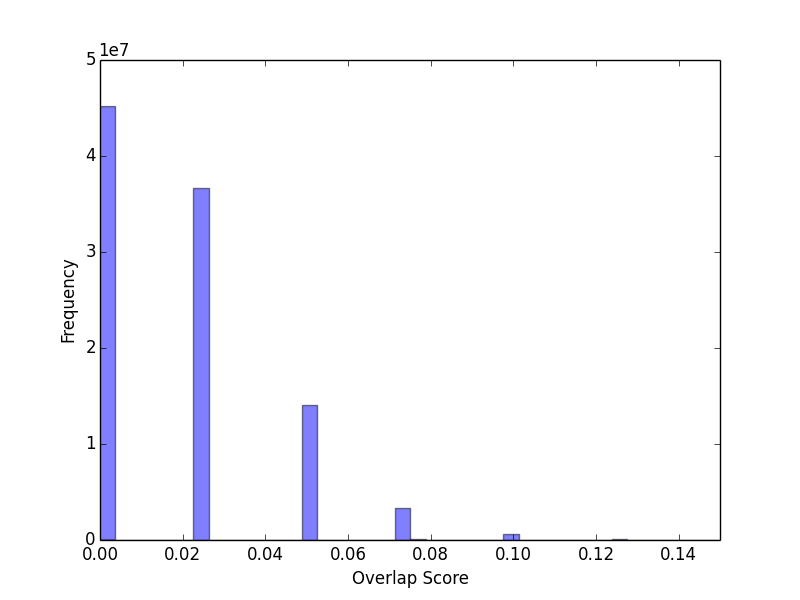
\includegraphics[scale=0.3]{EXP1_overlapScore.png}
				\label{fig4:a}
			}
			\subfloat[High-order scenario.]{%
				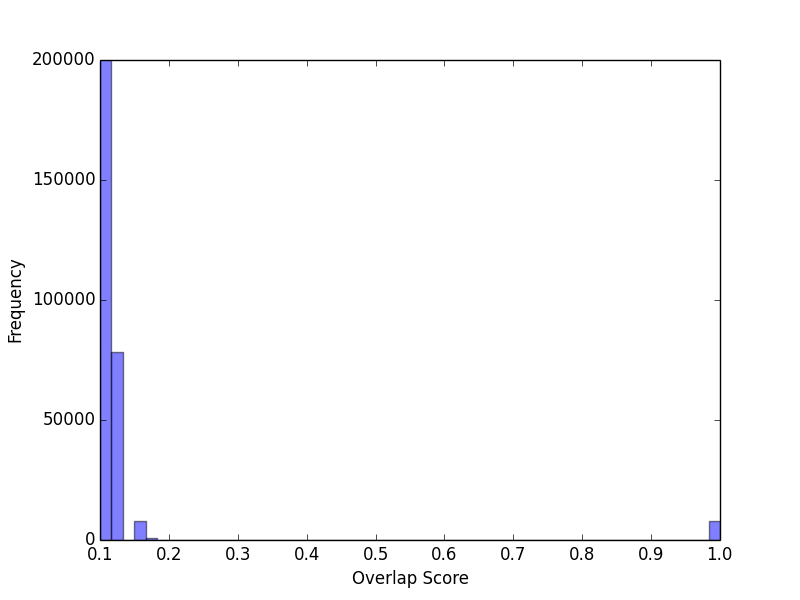
\includegraphics[scale=0.3]{EXP2_overlapScore.png}
				\label{fig4:b}
			}
			\caption{
                Distribution of overlap scores among SDRs in two scenarios:
                \emph{(a)} random, and \emph{(b)} high-order.
                Overlap between two SDRs in the random scenario is very low,
                which results in a distribution that decays around $10\%$.
                On the contrary, overlap among SDRs in the high-order scenario
                is larger, and in fact, given the way in which the dataset was
                constructed, some SDRs have perfect overlap.
			}
			\label{fig4}
		\end{figure}  
        

		The learning scenarios considered are:

        \begin{enumerate}
            \item\emph{Random sequences.} We generated $1000$ sequences, each sequence consists of $10$
            symbols taken at random, that is, by choosing $40$ columns at random out of a total of
            $2048$ columns. 
            This results in a sparse distributed representation (SDR) which is required as input for the TM.
            The process yields $10000$ random symbols with very low overlap among them.
            In this scenario at the beginning of each training epoch, we shuffle the set of sequences
            and then present each sequence to the TM until all have been processed.
            We repeat this for $N$ number of epochs ($N = 0$, $5$, 
            $10$, and $15$).
            A time-step is defined as a presentation of a single symbol from a sequence to the TM.
            Thus, by the end of simulation time we end up with a total number of time-steps equal to
            the number of epochs times the number of sequences times the number of symbols per sequence.
            This number is the temporal dimension of the tracked spike trains.
            In Fig.~\ref{fig4:a} we show the distribution of overlap scores obtained from estimating the
            overlap among all SDRs in this dataset.
            This distribution shows very low overlap among SDRs, which is expected given the random nature
            of the generation of these structures.
            \item\emph{High-order random sequences.} In the previous scenario we observed that the TM was able to 
            learn the sequences very fast due to the nature of the sequences used.
            There was no ambiguity nor high-order sequences that would have made necessary extensive
            periods of learning.
            To introduce ambiguity in the sequences we created a set of high-order sequences in the
            following way: we generate a random sequence $s$ consisting of $10$ SDRs, then we
            construct high-order sequence $s'$ by copying the contents of $s$ into $s'$ but substituting 
            the first and last symbols by random SDRs.
            We repeat this process for $500$ times which results in a total of 
            $1000$ sequences.
            The introduced ambiguity affected the accuracy of the TM as well as the structure of the
            pairwise correlations (see below).
            Figure \ref{fig4:b} shows the distribution of overlap scores among the SDRs generated in
            this particular scenario.
            As can be seen, the overlap scores are larger than in the random case, and in fact, there
            are SDRs with $100\%$ overlap. This results from the particular way in which sequences are
            constructed in this scenario.
            \item\emph{Real-world data.} In this scenario we use the NYC taxi dateset which consists
            of passenger count measured at different times of the day for a year period.
            In this scenario each time-step is defined as the presentation of a single measurement
            of the dataset, that is, a single passenger-count number.
            This yields $17520$ time-steps. Also, in this scenario there is no notion of epoch, that
            is, we present a single measurement to the TM only once.
            Figure \ref{fig5:a} shows the first $1000$ entries of this dataset. As can be seen, the data
            exhibits a recurring pattern of behaviour.
            As well, in this scenario we use a scalar encoder and spatial pooler in order to generate
            the appropriate set of SDRs to serve as input for the TM.
            In Fig.~\ref{fig5:c} we show the distribution of overlap scores for SDRs generated from the
            NYC taxi dataset.
            \item\emph{Periodic artificial data.} In this scenario we generate a sinusoidal function
            and we add random Gaussian noise. 
            In Fig.~\ref{fig5:b} we show an example of the sinusoidal function with noise added. 
            We consider $10000$ records sampled from this function.
            As with the previous scenario, we use a scalar encoder and
            a spatial pooler to generate appropriate SDRs to be fed to the TM.
            As well, here there is no notion of epoch as each record sampled from the sinusoidal function
            is presented once to the TM.
            Figure \ref{fig5:d} shows the distribution of overlap scores. As with the NYC taxi dataset, 
            the overlapping among SDRs is large and decays as it reaches unity.
            Large overlap scores are expected in periodic data as similar SDRs might occur in the data
            as time goes by.
        \end{enumerate}

        Will the particular shape of the distribution of overlap scores from our datasets have an impact
        on the shape of neural correlations?
        We will explore this question in the following sections.

		\begin{figure}[t]
			\centering
			\subfloat[NYC taxi dataset]{%
				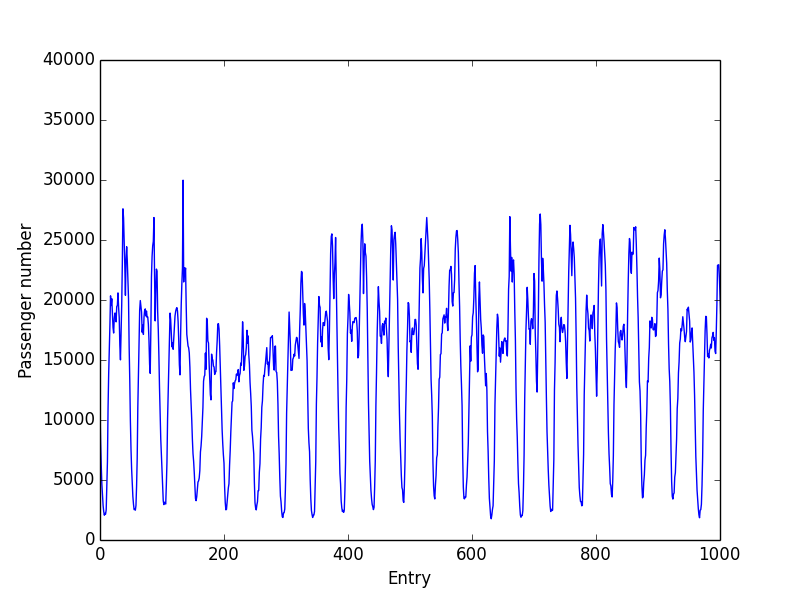
\includegraphics[scale=0.3]{EXP3_rawData.png}
				\label{fig5:a}
			}
			\subfloat[Noisy sinusoid function.]{%
				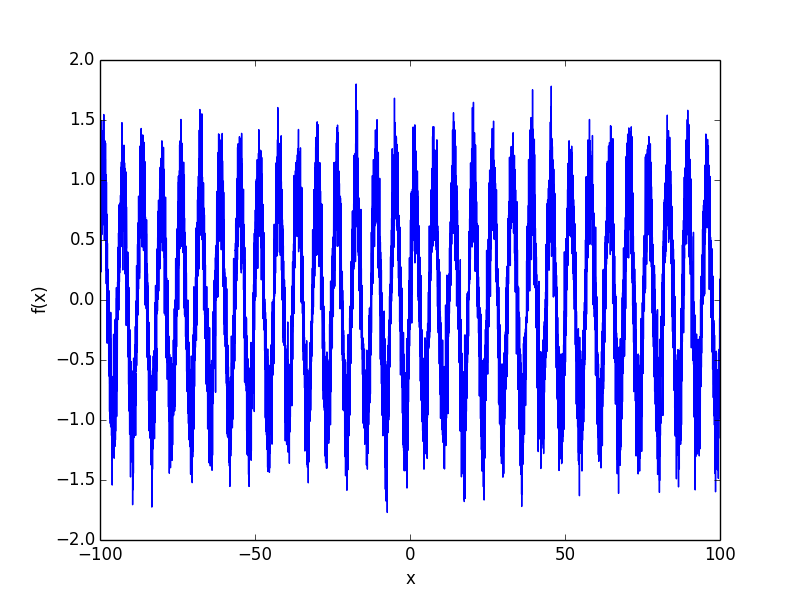
\includegraphics[scale=0.3]{EXP4_rawData.png}
				\label{fig5:b}
			}\\
			\subfloat[NYC taxi dataset]{%
				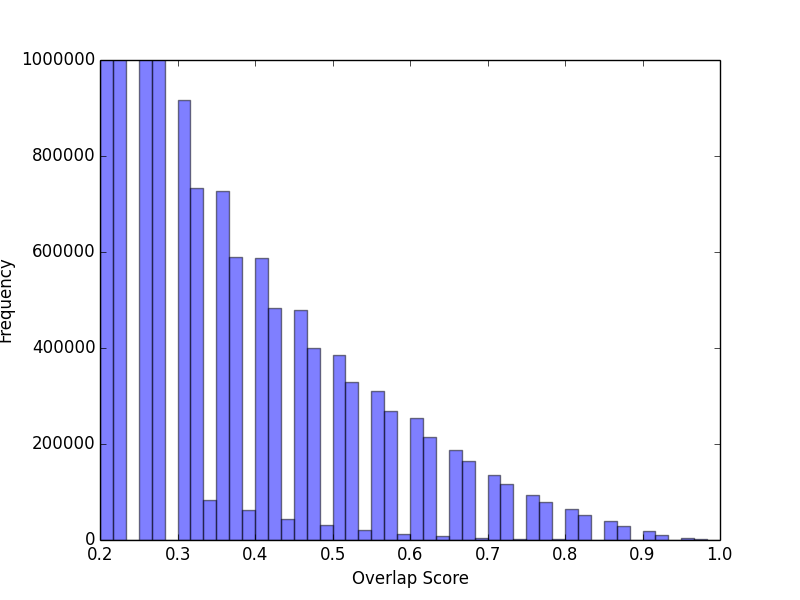
\includegraphics[scale=0.3]{EXP3_overlapScore.png}
				\label{fig5:c}
			}
			\subfloat[Noisy sinusoid function.]{%
				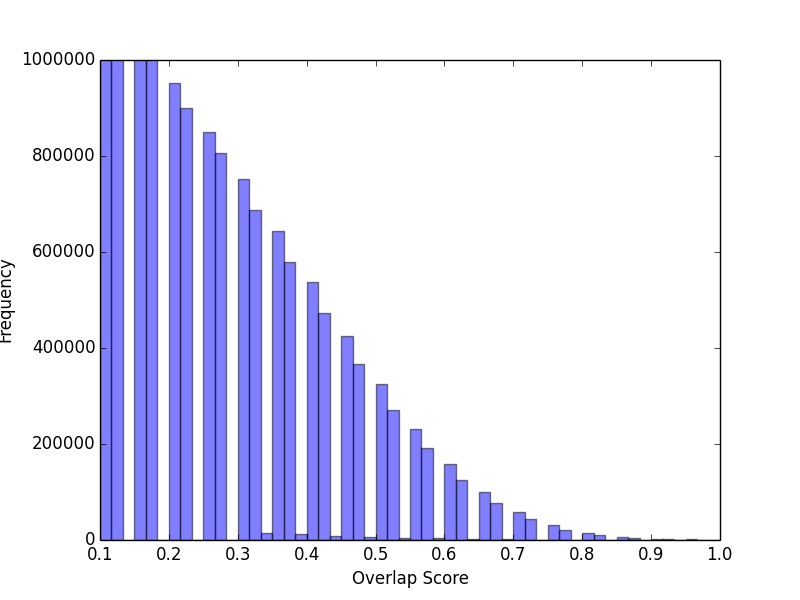
\includegraphics[scale=0.3]{EXP4_overlapScore.png}
				\label{fig5:d}
			}			
			\caption{
                Raw data and overlap score distribution for two scenarios:
                \emph{(a)}, \emph{(c)} NYC taxi dataset, and \emph{(b)}, \emph{(d)}
                noisy sinusoid function.
                Both datasets are periodic, and this fact is captured by the distribution
                of overlap scores among SDRs.
			}
			\label{fig5}
		\end{figure}  
		
		
    \section{Results}
        \subsection{Pairwise correlations are small}    
            Pairwise correlations were estimated by subsampling the spike trains obtained from tracking activations in all
            cells. The number of cells considered in the sample was $1000$; and we considered time windows of $1000$ time
            steps of duration, that is, every $1000$ time steps of simulation time we sampled $1000$ cells from the TM and
            considered its spike trains in the last $1000$ time steps.
            Correlations were computed by estimating the Pearson correlation coefficient (PCC) between all neuron pairs in the
            sample. 
            Next, we considered the distribution of such pairwise correlation coefficients.

            In all scenarios considered the distribution of pairwise correlations exhibit weak correlations among neuron pairs.
            For instance, in Fig.~\ref{fig6} we show the distribution of pairwise correlations for the random scenario.
            Here, we can see how most pairwise correlations are small: no greater than $0.10$, and also there are positive as
            well as negative correlations.
            There are correlations larger than those but occur so few times that they might be considered outliers.
            This behaviour was also observed in the high-order random scenario, in which sequences possess a large overlap score
            among each other.
            In Fig.~\ref{fig7} we present the distribution of pairwise correlations for the high-order scenario.
            
            What is the effect of learning over the nature of pairwise correlations?
            In the case of the random and high-order scenarios, we observed that the effects of presenting the 
            TM with repeated presentations of the same sequences for the purpose of learning (i.e. $epochs>0$)
            had an impact over the quality of the distribution of pairwise correlations.
            As training times become larger the distribution shrinks in the sense that positive pairwise correlations
            decrease (see Fig.~\ref{fig11-3}).
          

		    \begin{figure}[t]
			    \centering
			    \subfloat[$epochs = 1$]{%
				    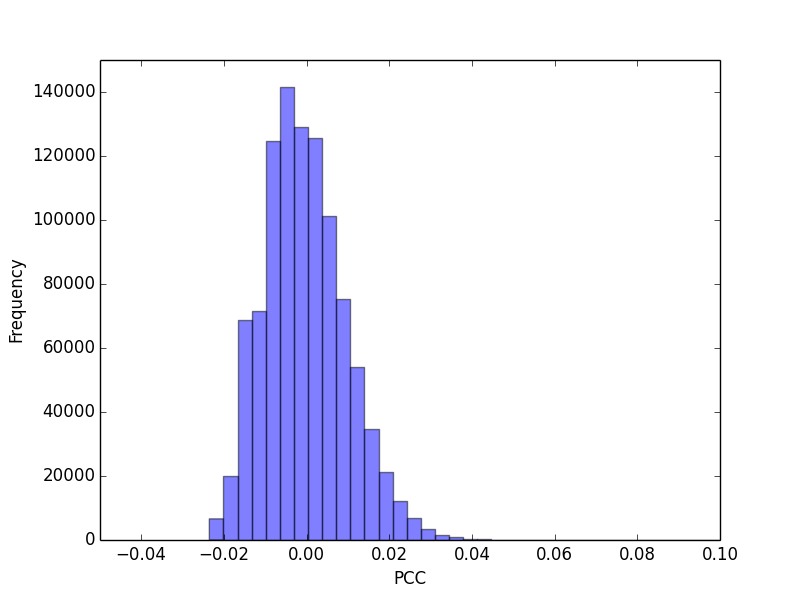
\includegraphics[scale=0.3]{EXP1_PCC_1ts.png}
				    \label{fig6:a}
			    }
			    \subfloat[$epochs = 5$]{%
				    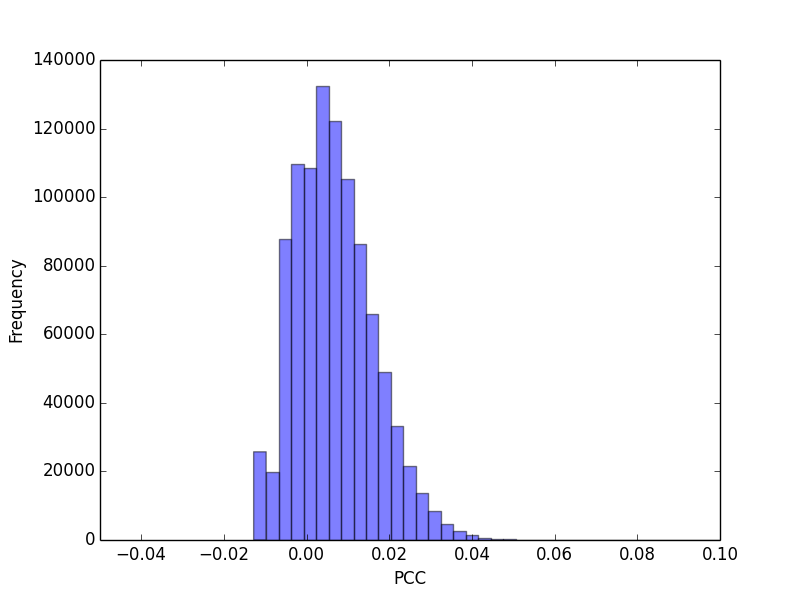
\includegraphics[scale=0.3]{EXP1_PCC_5ts.png}
				    \label{fig6:b}
			    }\\
			    \subfloat[$epochs = 10$]{%
    				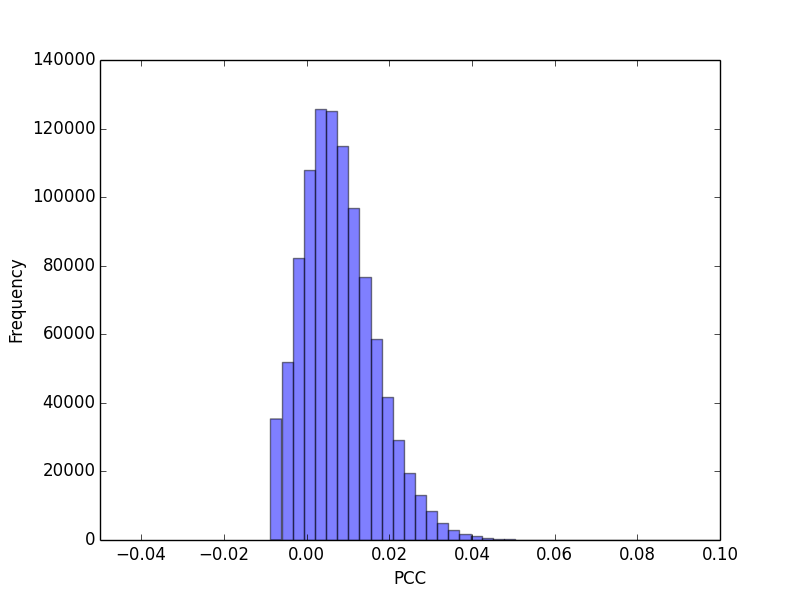
\includegraphics[scale=0.3]{EXP1_PCC_10ts.png}
	    			\label{fig6:c}
		    	}
			    \subfloat[$epochs = 15$]{%
				    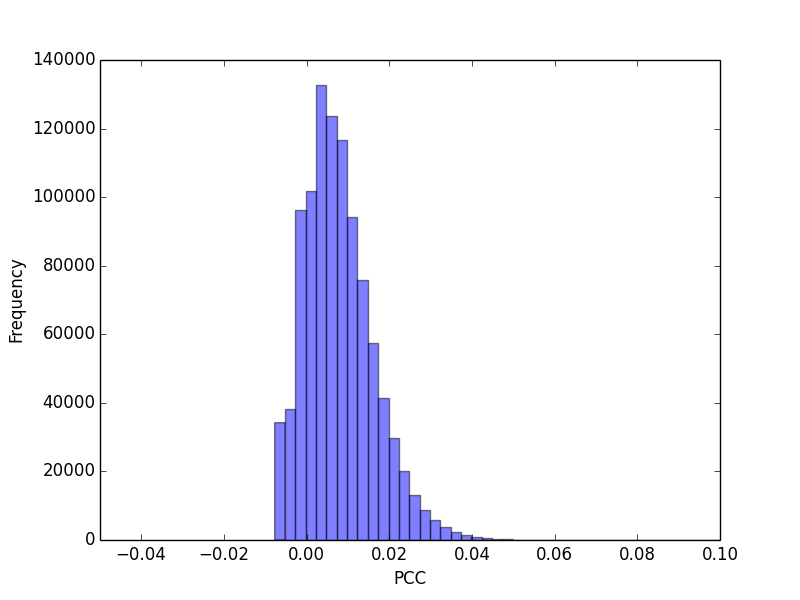
\includegraphics[scale=0.3]{EXP1_PCC_15ts.png}
				    \label{fig6:d}
			    }			
			    \caption{
			        Distribution of pairwise correlations as estimated by the Pearson
			        correlation coefficient of spike trains of neuron pairs for the random
			        scenario.
			        Here we also show the shape of the distribution as we increase the training periods (epochs)
			        of the TM when presented with this particular dataset.
			    }
			    \label{fig6}
		    \end{figure} 

		    \begin{figure}[t]
			    \centering
			    \subfloat[$epochs = 1$]{%
				    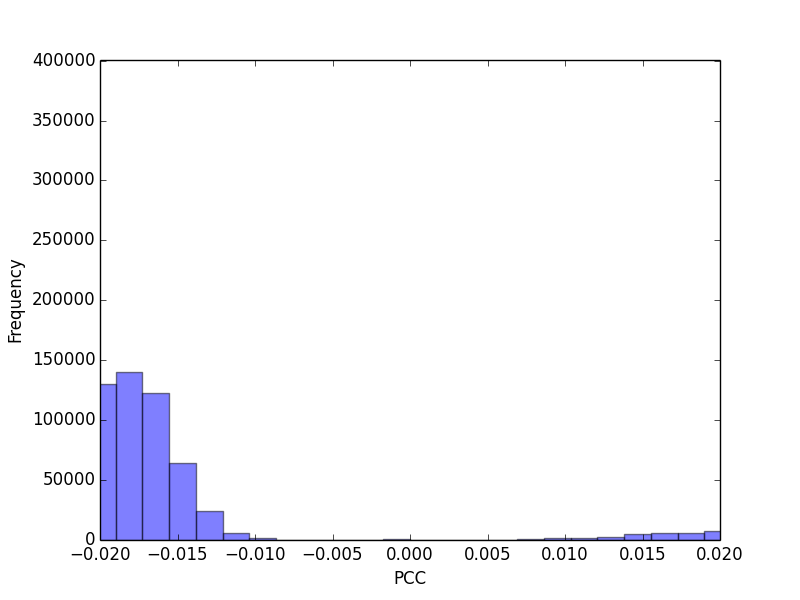
\includegraphics[scale=0.3]{EXP2_PCC_1ts.png}
				    \label{fig7:a}
			    }
			    \subfloat[$epochs = 5$]{%
				    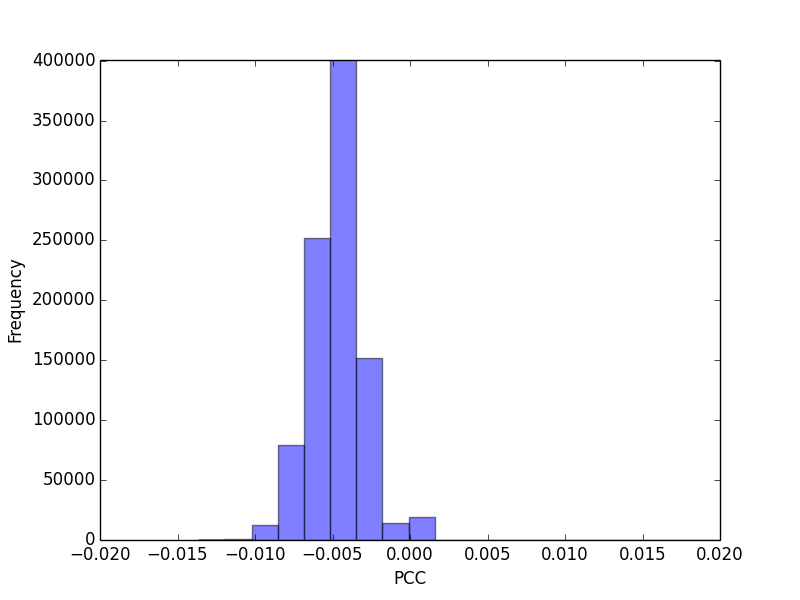
\includegraphics[scale=0.3]{EXP2_PCC_5ts.png}
				    \label{fig7:b}
			    }\\
			    \subfloat[$epochs = 10$]{%
    				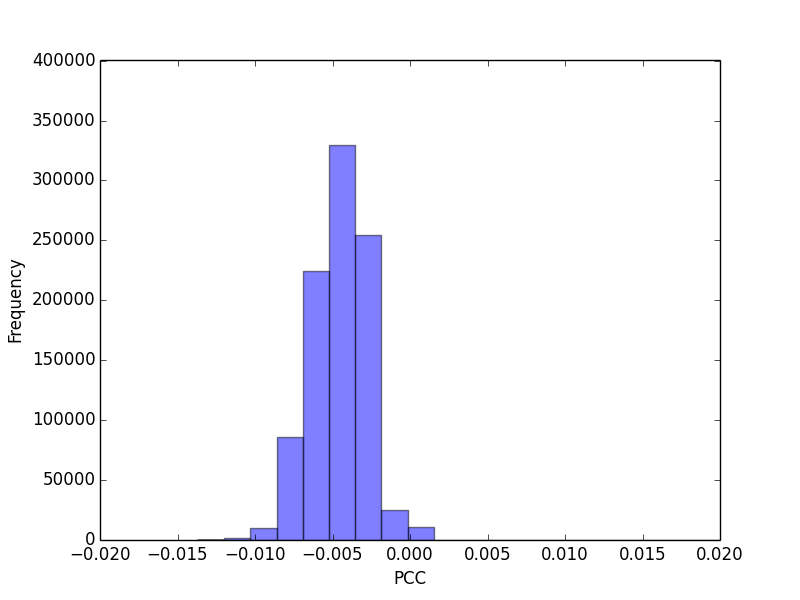
\includegraphics[scale=0.3]{EXP2_PCC_10ts.png}
	    			\label{fig7:c}
		    	}
			    \subfloat[$epochs = 15$]{%
				    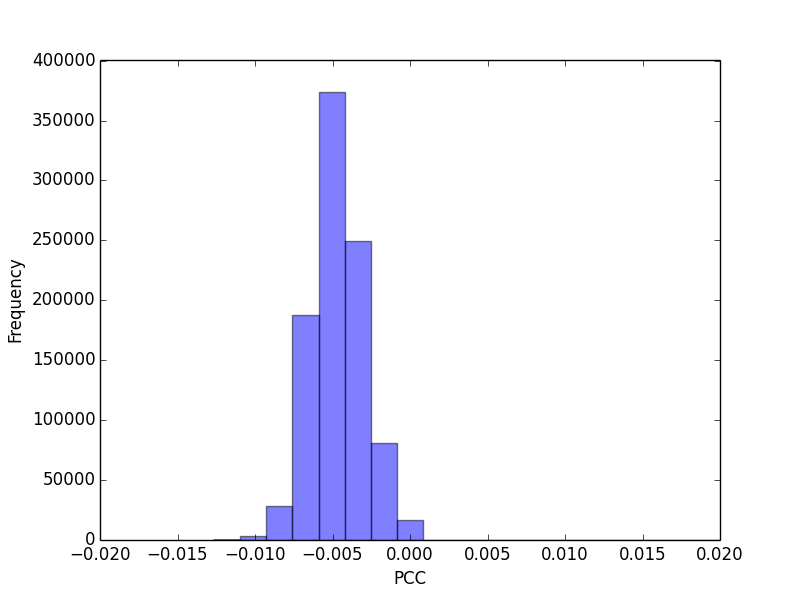
\includegraphics[scale=0.3]{EXP2_PCC_15ts.png}
				    \label{fig7:d}
			    }			
			    \caption{
			        Same as Fig.~\ref{fig6} for the high-order scenario.
			    }
			    \label{fig7}
		    \end{figure}		    
            
            For the other scenarios, NYC taxi dataset and the noisy sinusoid, the shape of the distribution
            of pairwise correlations looks different.
            In both cases although there are no training periods larger than one for the TM, we do have them for the spatial pooler (SP)
            which will refine the process of generating SDRs from numerical values.
            Increasing training times in the SP stage has the effect of making SDRs more resilient to noise,
            which has the following consequence: similar input values will be mapped to similar SDRs.
            This process indeed results in changes in the shape of the distribution of pairwise correlations, as well
            as in the distribution of columns that become active during simulation time: the \emph{column usage}.
            
            For instance, in Fig.~\ref{fig8} we show how the number of records used for training the SP
            affects the distribution of column usage in the TM. As more items are used to train the SP, the
            less number of columns remain idle during simulation time.

		    \begin{figure}[t]
			    \centering
			    \subfloat[$5,000$ training items]{%
				    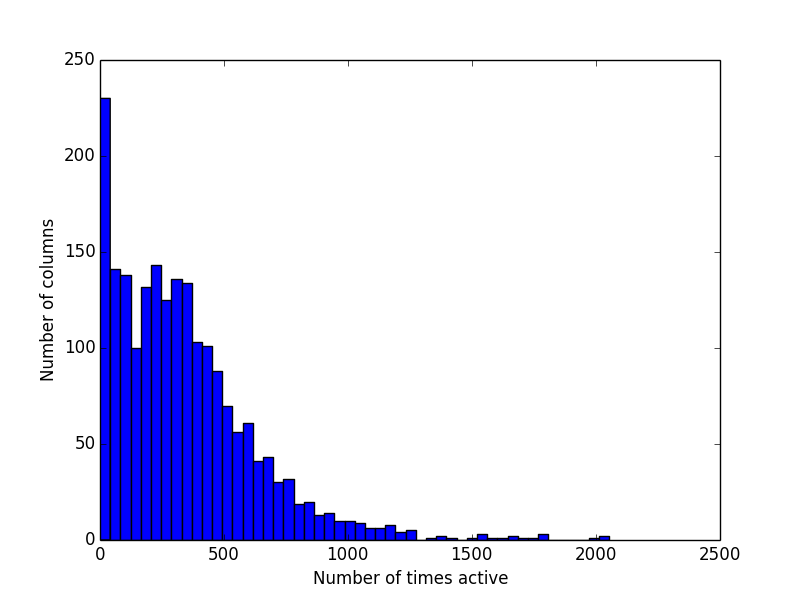
\includegraphics[scale=0.3]{EXP3_colUsage_5k.png}
				    \label{fig8:a}
			    }
			    \subfloat[$10000$ training items]{%
				    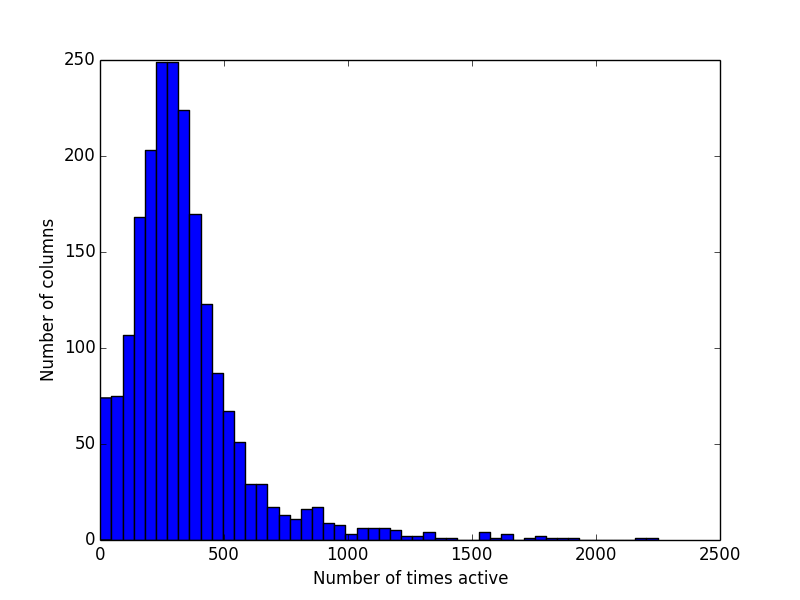
\includegraphics[scale=0.3]{EXP3_colUsage_10k.png}
				    \label{fig8:b}
			    }\\
			    \subfloat[$15,000$ training items]{%
    				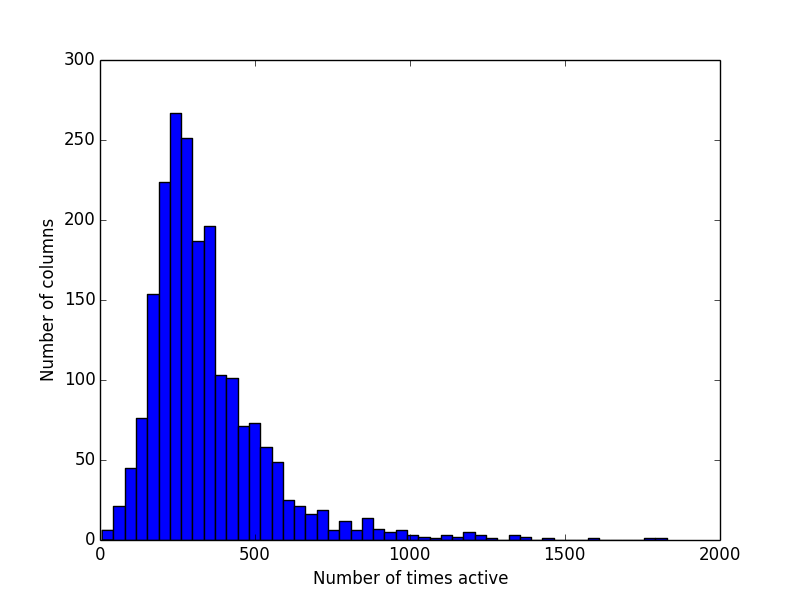
\includegraphics[scale=0.3]{EXP3_colUsage_15k.png}
	    			\label{fig8:c}
		    	}
			    \caption{
			        Distribution of active columns or column usage in the TM. The $x$
			        axis represent the number of times that a column has
			        been active during simulation time.
			        As we varied the number of training items for the SP,
			        the number of idle columns decrease.
			    }
			    \label{fig8}
		    \end{figure}

            The same behaviour is observed in the noisy sinusoid scenario (see Fig.~\ref{fig9}).
            Naturally, the column usage is related to the correlated activity within the TM;
            thus, the shape of the distribution of column usage is also correlated with the shape of the
            distribution of pairwise correlations.
		    

		    \begin{figure}[t]
			    \centering
			    \subfloat[$1000$ training items]{%
				    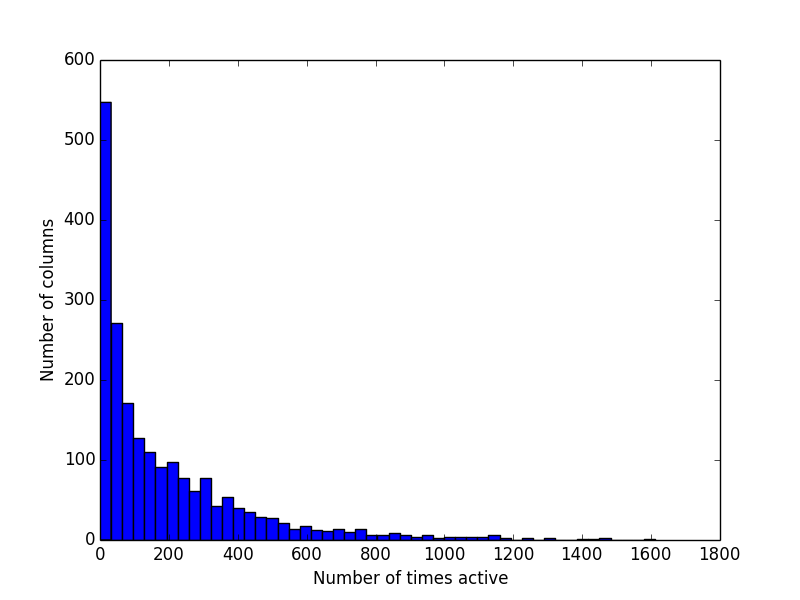
\includegraphics[scale=0.3]{EXP4_colUsage_1k.png}
				    \label{fig9:a}
			    }
			    \subfloat[$5,000$ training items]{%
				    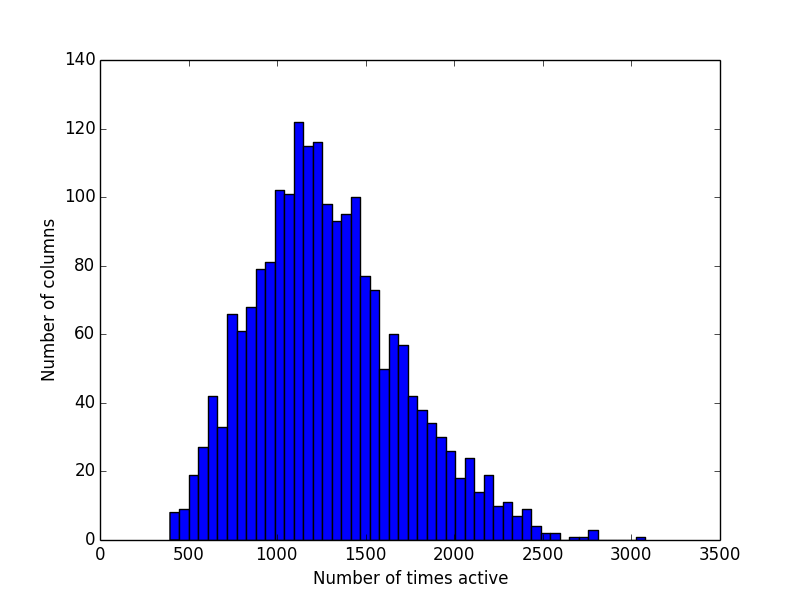
\includegraphics[scale=0.3]{EXP4_colUsage_4k.png}
				    \label{fig9:b}
			    }\\
			    \subfloat[$10000$ training items]{%
    				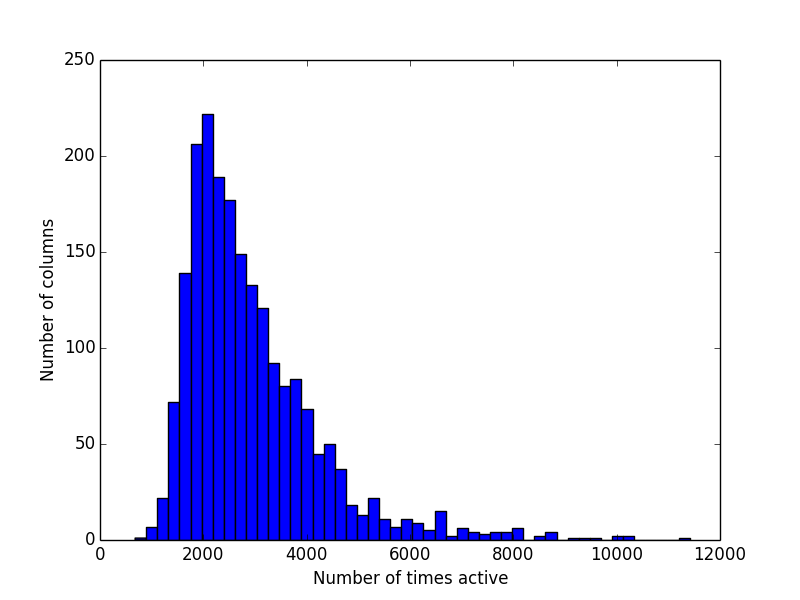
\includegraphics[scale=0.3]{EXP4_colUsage_10k.png}
	    			\label{fig9:c}
		    	}
			    \caption{
			        Same as Fig.~\ref{fig8} for the noisy sinusoid scenario.
			        The number of items used to train the SP result in different
			        shapes in the distribution of column usage in the TM.
			        %This eventually affects the shape of the neural correlations.
			    }
			    \label{fig9}
		    \end{figure}
		    
		    In Figure \ref{fig10} we show the distribution of pairwise correlations from the TM
		    for the NYC taxi dataset and for different number of training items in the SP.
		    As can be seen in this image, the mode of the distribution is around a negative value,
		    whose frequency becomes larger as more records are included in the training set for the
		    SP.
		    Unlike the random and high-order cases, the distribution exhibits a larger left-tail
		    which implies the non-negligible existence of negative correlations.
		    As well, this distribution exhibits a slowly decaying right-tail which is larger
		    than in the random and high-order cases.
		    In any case, pairwise correlations are weak, and in most cases negative.
		    For instance, compare Fig.~\ref{fig6:d} with \ref{fig10:c}.
		    In the former, negative correlations barely exist and the distribution
		    does not exhibit any slowly-decaying right-tail.
		    
		    
		    \begin{figure}[t]
			    \centering
			    \subfloat[$5,000$ training items]{%
				    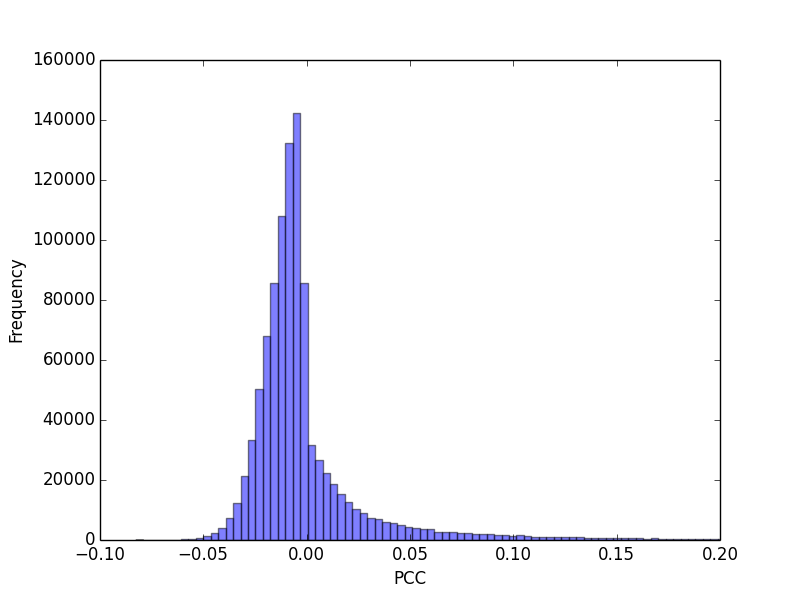
\includegraphics[scale=0.3]{EXP3_PCC_5k.png}
				    \label{fig10:a}
			    }
			    \subfloat[$10000$ training items]{%
				    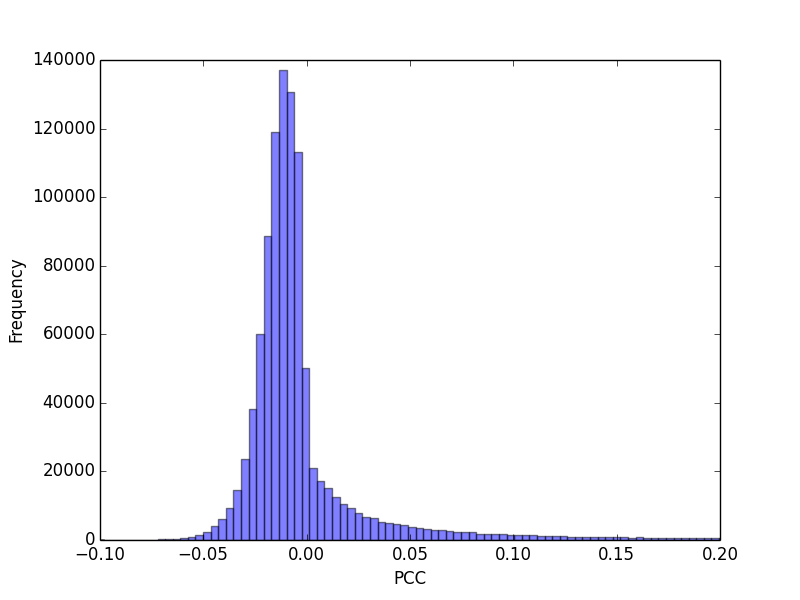
\includegraphics[scale=0.3]{EXP3_PCC_10k.png}
				    \label{fig10:b}
			    }\\
			    \subfloat[$15,000$ training items]{%
    				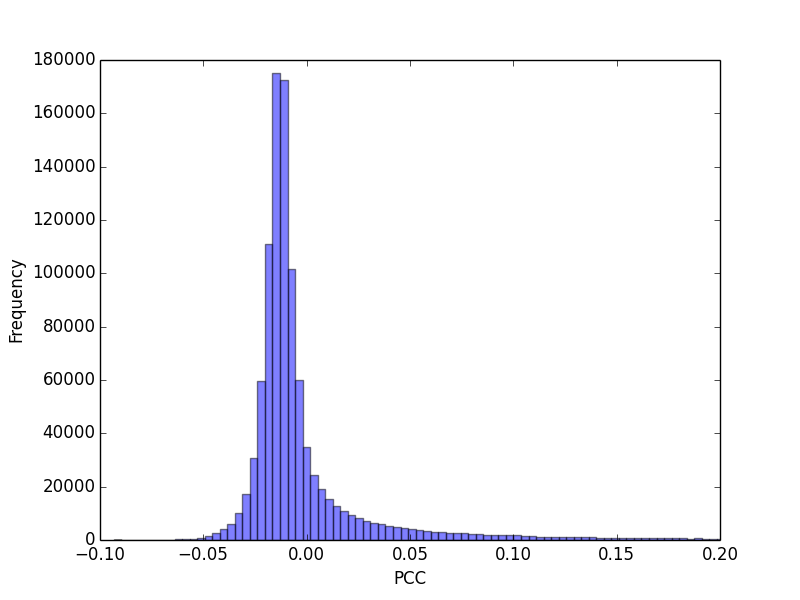
\includegraphics[scale=0.3]{EXP3_PCC_15k.png}
	    			\label{fig10:c}
		    	}
			    \caption{
			        Distribution of pairwise neural correlations for the NYC taxi dataset and
			        different numbers of records used as training set for the SP.
			        Unlike previous cases, this distribution exhibits slow decaying tails.
			    }
			    \label{fig10}
		    \end{figure}	
		    
		    A similar behaviour is observed in the correlated activity of the TM when using the
		    noisy sinusoid dataset as input.
		    However in this case a sharp transition between positive and negative correlations
		    can be noticed (see Fig.~\ref{fig11}).
		    Negative correlations abound as in the case of the NYC taxi dataset; also, as in the
		    latter case, left and right tails can be identified in the distribution.

		    \begin{figure}[t]
			    \centering
			    \subfloat[$1000$ training items]{%
				    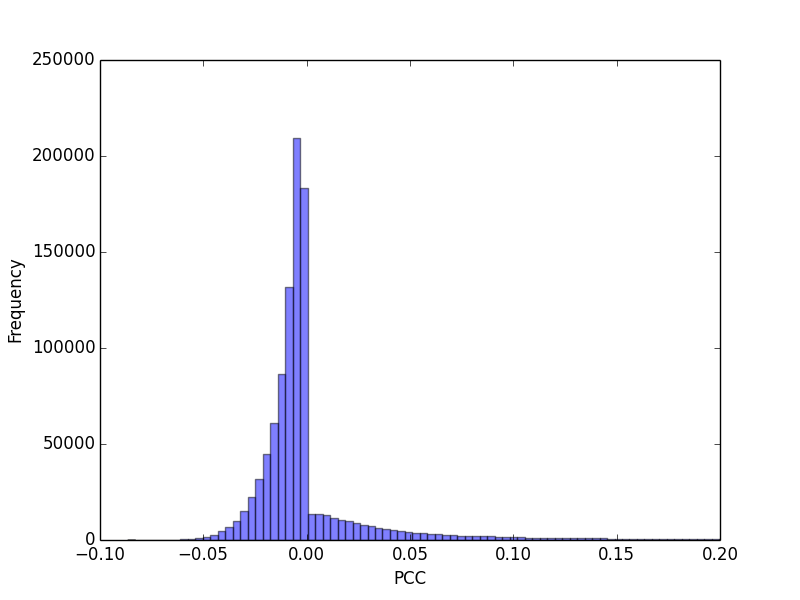
\includegraphics[scale=0.3]{EXP4_PCC_1k.png}
				    \label{fig11:a}
			    }
			    \subfloat[$4,000$ training items]{%
				    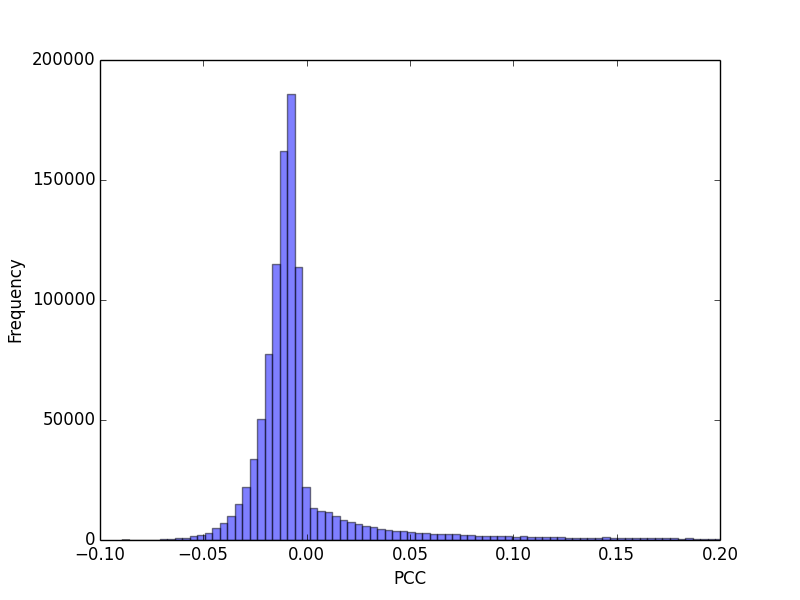
\includegraphics[scale=0.3]{EXP4_PCC_5k.png}
				    \label{fig11:b}
			    }\\
			    \subfloat[$10000$ training items]{%
    				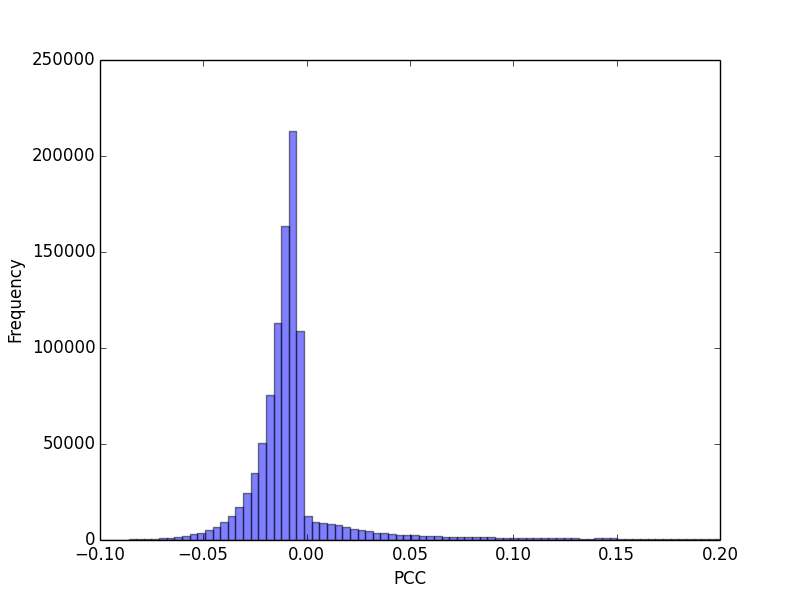
\includegraphics[scale=0.3]{EXP4_PCC_10k.png}
	    			\label{fig11:c}
		    	}
			    \caption{
			        Same as Fig.~\ref{fig10} for the noisy sinusoid dataset.
			    }
			    \label{fig11}
		    \end{figure}
		    
		    We hypothesize that the particular behaviour of these periodic scenarios, namely
		    the NYC taxi and the noisy sinusoid datasets, is related to the particular
		    nature of the input stimulus.
		    The periodic nature of the dataset affects the overlap scores among SDRs in
		    these two datasets (see Fig.~\ref{fig5}).
		    This ultimately affect the nature of the neural correlations.
		    For instance, we would expect that as the TM learns, negative correlations
		    start to emerge as the process of learning in the TM implies that cells
		    within columns will be silent while one other cell from the same column
		    is active in order to represent the current input.
		    This means that cells within columns will become negatively correlated
		    as the TM learns a sequence.
		    
		    What are the effects of increasing the training periods of the TM for
		    the NYC taxi and the noisy sinusoid datasets?
		    For this purpose, we present the dataset in repeated occasions to the
		    TM, and keep track of the evolution of the distribution of pairwise
		    neural correlations.

            In Fig.~\ref{fig11-1} we present the distribution of pairwise correlations
            for the NYC taxi dataset at two different stages of learning: one at
            $1000$ time-steps when the TM is at the early stages of learning, 
            and another at $51,000$ time-steps when the TM is completing 3 epochs
            of learning.
            
            Unlike the random and high-order scenarios, the negative correlations
            do not vanish, nor the distribution shrinks.
            On the contrary, negative correlations abound possibly as a result of
            the periodic nature of the dataset.
            
		    \begin{figure}[t]
			    \centering
			    \subfloat[TM at time-step $1000$]{%
				    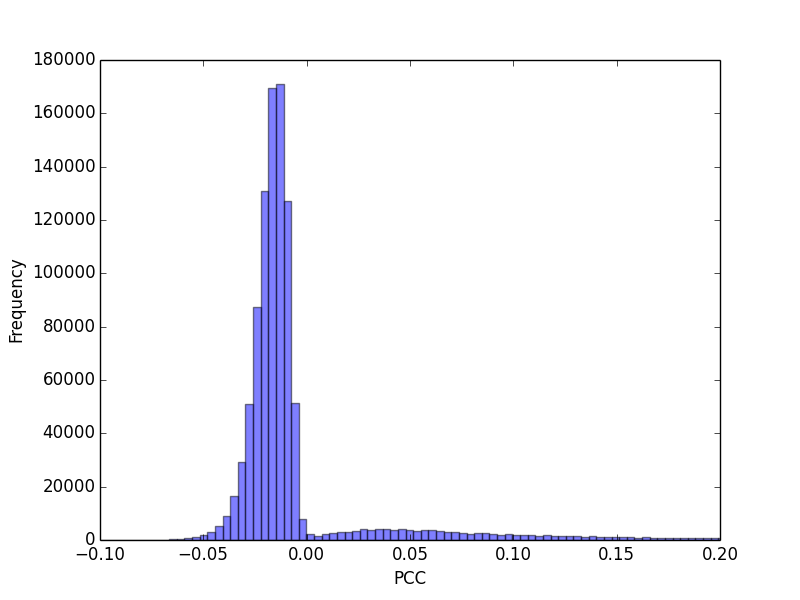
\includegraphics[scale=0.3]{EXP3_1k_stepsTM.png}
				    \label{fig11-1:a}
			    }
			    \subfloat[TM at time-step $51,000$]{%
				    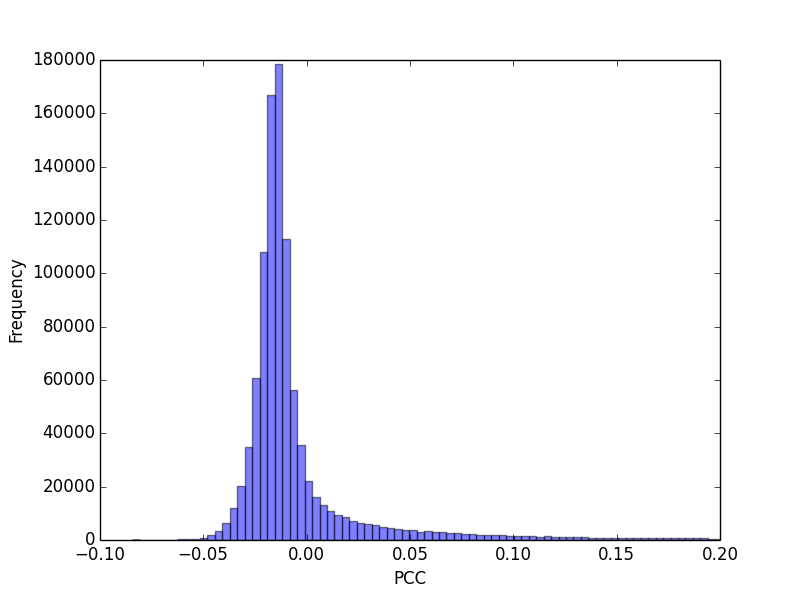
\includegraphics[scale=0.3]{EXP3_51k_stepsTM.png}
				    \label{fig11-1:b}
			    }
			    \caption{
			        Distribution of pairwise correlations for the NYC taxi dataset.
			        Here we increased the training periods of the TM by presenting 3 times
			        the whole dataset. In \emph{(a)} we show the distribution at the
			        first stages of learning, whereas in \emph{(b)} we present it at
			        the last stages. As can be seen, negative correlations do not
			        vanish as learning periods increase.
			    }
			    \label{fig11-1}
		    \end{figure}

            A similar behaviour is observed in the noisy sinusoid dataset.
            As training periods in the TM increase, the right tail becomes more evident.
            Negative correlations do not vanish as occurs with the random and 
            high-order scenarios, which again can be related to the periodic nature
            of the dataset.

		    \begin{figure}[t]
			    \centering
			    \subfloat[TM at time-step $1000$]{%
				    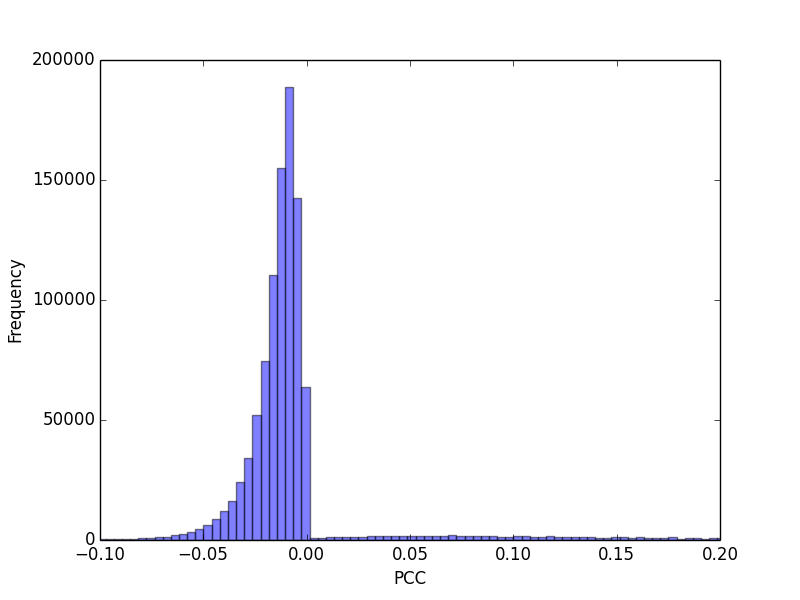
\includegraphics[scale=0.3]{EXP4_1k_stepsTM.png}
				    \label{fig11-2:a}
			    }
			    \subfloat[TM at time-step $29,000$]{%
				    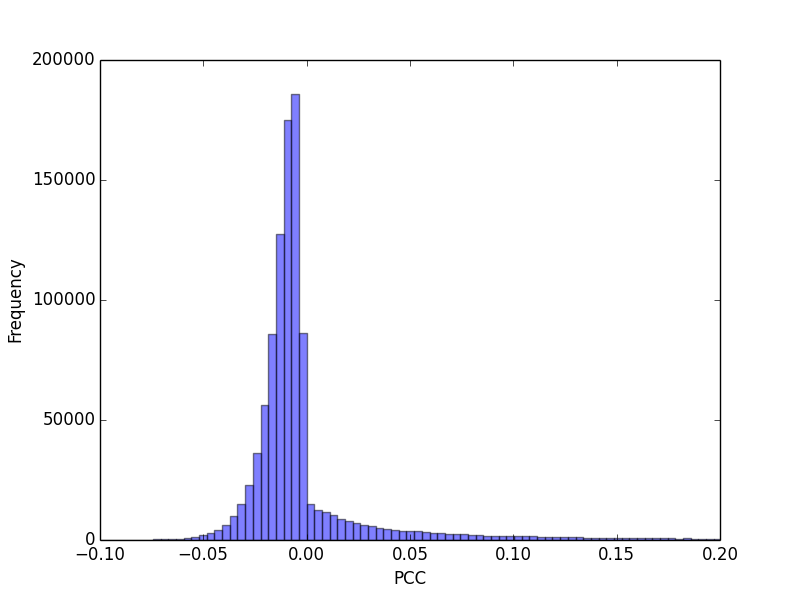
\includegraphics[scale=0.3]{EXP4_29k_stepsTM.png}
				    \label{fig11-2:b}
			    }
			    \caption{
			        Similar to Fig.~\ref{fig11-1} for the noisy sinusoid dataset.
                    In \emph{(a)} we show the distribution at the
			        first stages of learning, whereas in \emph{(b)} we present it at
			        the last stages. As can be seen, negative correlations do not
			        vanish as learning periods increase.
			    }
			    \label{fig11-2}
		    \end{figure}

		    \begin{figure}[t]
			    \centering
			    \subfloat[Random]{%
				    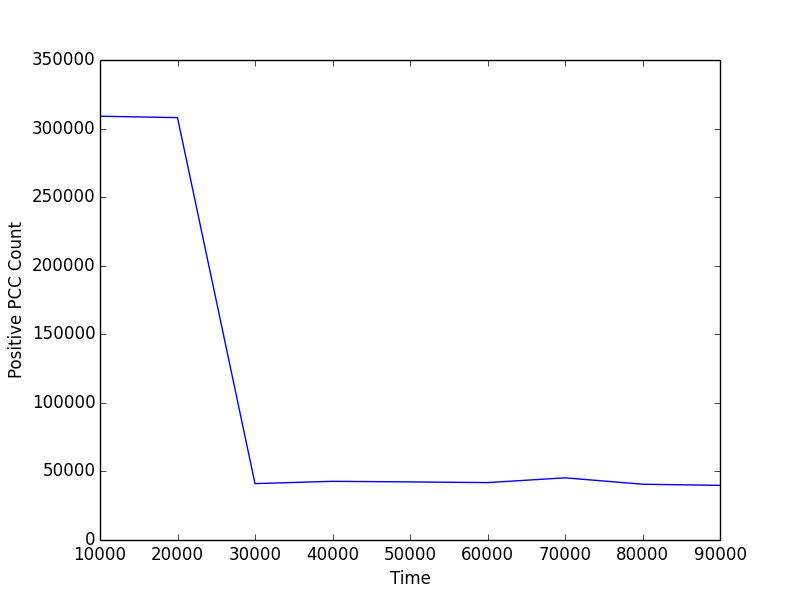
\includegraphics[scale=0.3]{EXP1_positivePCCTrace.png}
				    \label{fig11-3:a}
			    }
			    \subfloat[High-order]{%
				    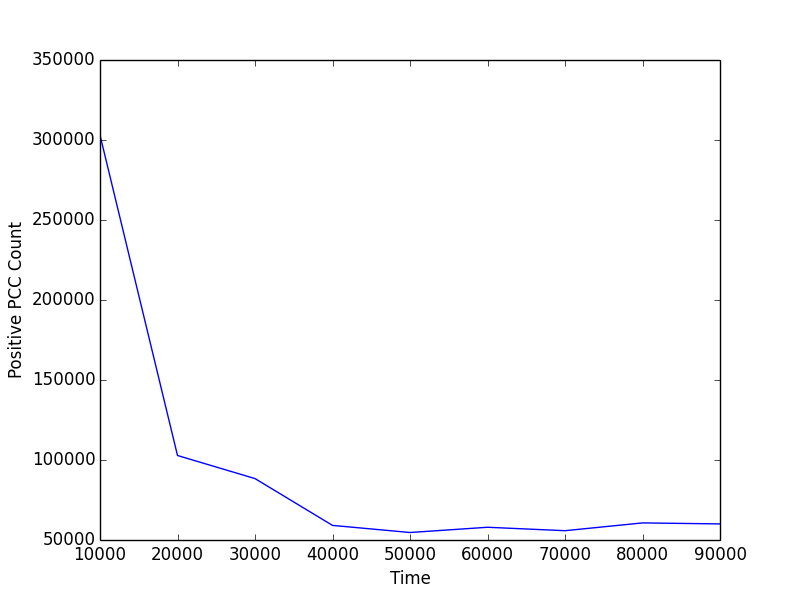
\includegraphics[scale=0.3]{EXP2_positivePCCTrace.png}
				    \label{fig11-3:b}
			    }\\
			    \subfloat[NYC taxi dataset]{%
    				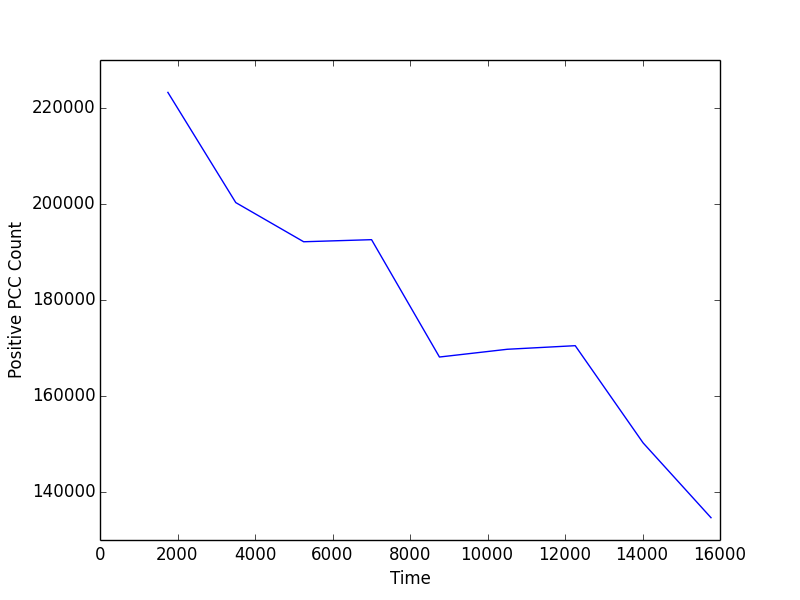
\includegraphics[scale=0.3]{EXP3_positivePCCTrace.png}
	    			\label{fig11-3:c}
		    	}
			    \subfloat[Noisy sinusoid]{%
				    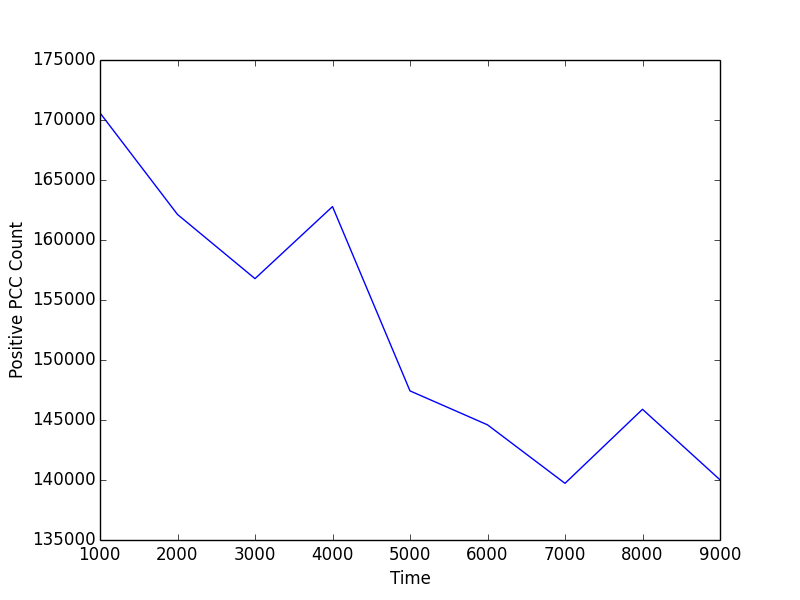
\includegraphics[scale=0.3]{EXP4_positivePCCTrace.png}
				    \label{fig11-3:d}
			    }			
			    \caption{
			        Trace of amount of positive pairwise correlations for all experiments.
			        The number of positive correlations decrease as learning increases in the TM.
			        This implies that correlations are becoming weaker as learning progresses.
			    }
			    \label{fig11-3}
		    \end{figure} 
		    

        \subsection{Network states are strongly correlated}
            Following the study of Schneidman and colleagues~\cite{schneidman2006weak} we enquired about the
            frequency that binary patterns encoded by synchronous activation of a group of $N$ neurons occur
            in the network as a result of stimulus presentation.
            The motivation behind this kind of analysis is to reveal whether weak pairwise correlations might
            have an overall effect on population coding when considering higher-order correlations or anticorrelations,
            and comparing them against a random model.
            In other words, this analysis serves as a proxy to study higher-order correlations within a population
            as well as a first step to study how a population of cells encode information.
            For instance, a binary pattern $x$ of length $N$ occurring more often than predicted by a random model 
            might carry neural information relevant to the organism.
            This is what is meant by network states in the work of Schneidman and 
            co-workers~\cite{ganmor2015thesaurus,schneidman2006weak}.

			Fig.~\ref{fig12} shows an example of a raster plot obtained by subsampling $N =10$ cells from the spike trains
			of the TM.
			Because in our experiments we are working with discrete time there is no need to consider a $\Delta t$ window
			of time to count spikes as in Refs.~\cite{schneidman2006weak,berkes2011spontaneous}.
			Therefore, we can build a binary pattern from spike trains by consider the activity of $N$ subsampled cells
			at time-step $t$.
			Ten cells make a binary pattern of length $10$ in which the $i$-th entry is $1$ if the $i$-th cell is active
			at time $t$, and zero otherwise.

 		    \begin{figure}[t]
			    \centering
			    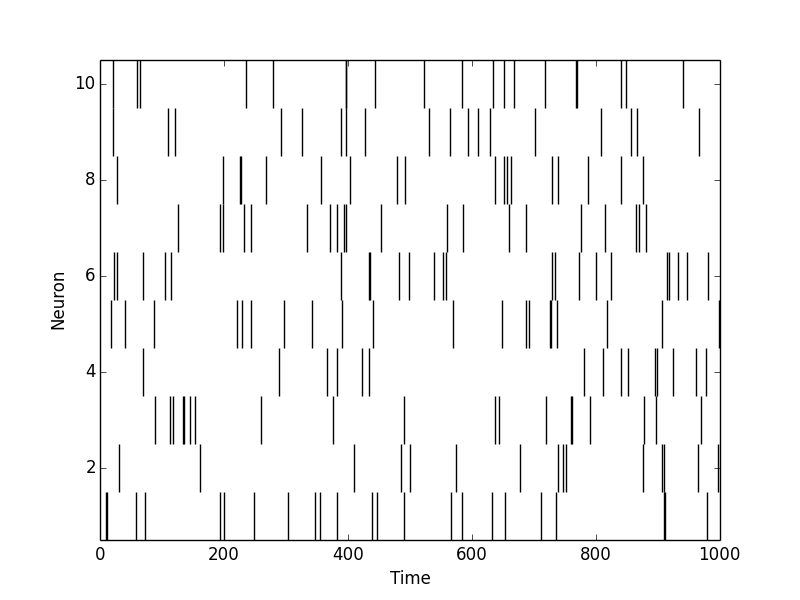
\includegraphics[scale=0.5]{rasterTM_10cells_1kTS.png}
			    \caption{
                    Raster plot of $10$ cells in the TM for $1000$ time-steps.
				    A binary pattern is formed by considering the synchronous activation
				    of cells in a discrete time-step $t$.
			    }
			    \label{fig12}
		    \end{figure}
		
			For the random and high-order scenarios, the ``spiking'' activity of a TM in the early stages of 
			learning resembles the activity of a Poisson
			spiking model with mean firing rate of $18$ spikes per second\footnote{In our
			simulations, a discrete time-step denotes a millisecond. Therefore $1000$ time-steps result in a
			second of simulation.}.
            Figure \ref{fig13} shows raster plots of sampled cells from the TM and from the Poisson spiking model.
            The activity from both models is practically indistinguishable, suggesting that the TM behaves like
            a random spiking model as the TM starts to learn sequences.

		    \begin{figure}[t]
			    \centering
			    \subfloat[Temporal Memory]{%
				    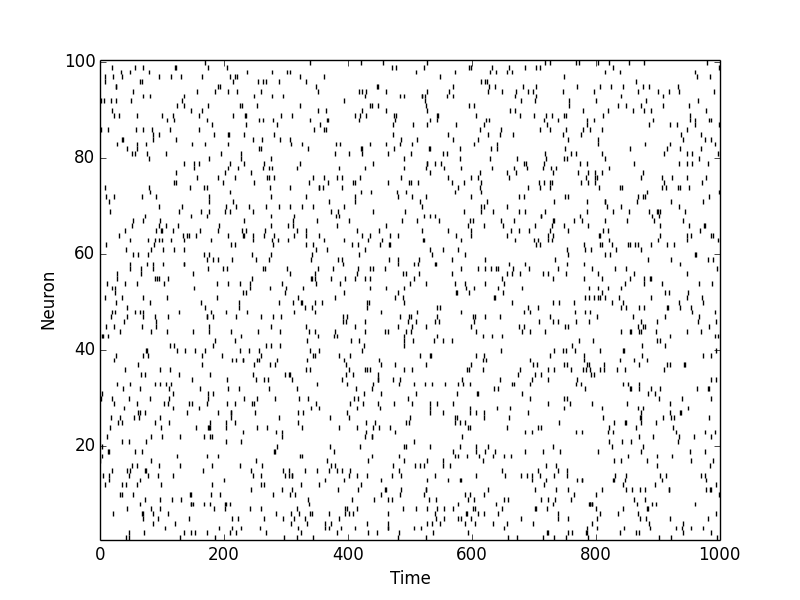
\includegraphics[scale=0.3]{EXP1_rasterTM.png}
				    \label{fig13:a}
			    }
			    \subfloat[Poisson model]{%
				    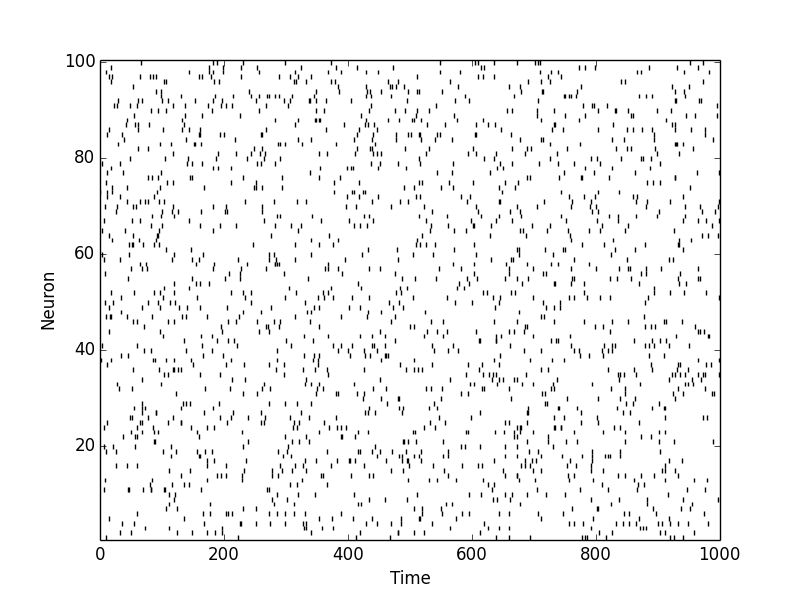
\includegraphics[scale=0.3]{EXP1_rasterPoisson.png}
				    \label{fig13:b}
			    }
			    \caption{
			        Raster plots of $100$ cells sampled from \emph{(a)} the TM, and
			        \emph{(b)} a Poisson spiking model.
			        The activity from both models is practically indistinguishable.
			    }
			    \label{fig13}
		    \end{figure}

			We estimated the distribution of waiting times also known as inter-spike intervals (ISI) by sampling
			the activity of $1000$ random cells in the TM, and then estimating the distribution of the time-steps
			in-between two spikes in such sample.
			The same process was repeated with the Poisson model, although in this case the spiking of $1000$ cells
			was generated \emph{ex profeso}.
            In Fig.~\ref{fig14} we present the distribution of inter-spike intervals of both models.
            As can be seen, these distributions are nearly identical.

		    \begin{figure}[t]
			    \centering
			    \subfloat[ISI distribution of TM]{%
				    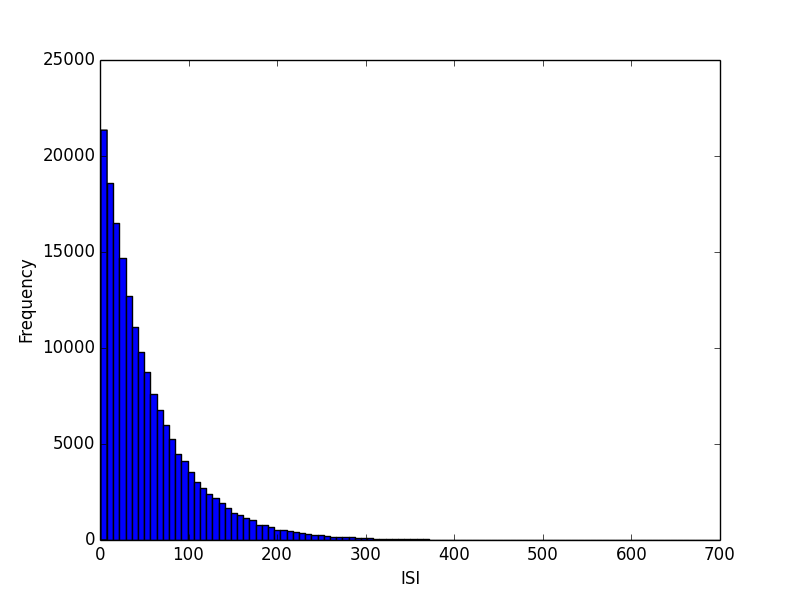
\includegraphics[scale=0.3]{EXP1_isiTM.png}
				    \label{fig14:a}
			    }
			    \subfloat[ISI distribution of Poisson model]{%
				    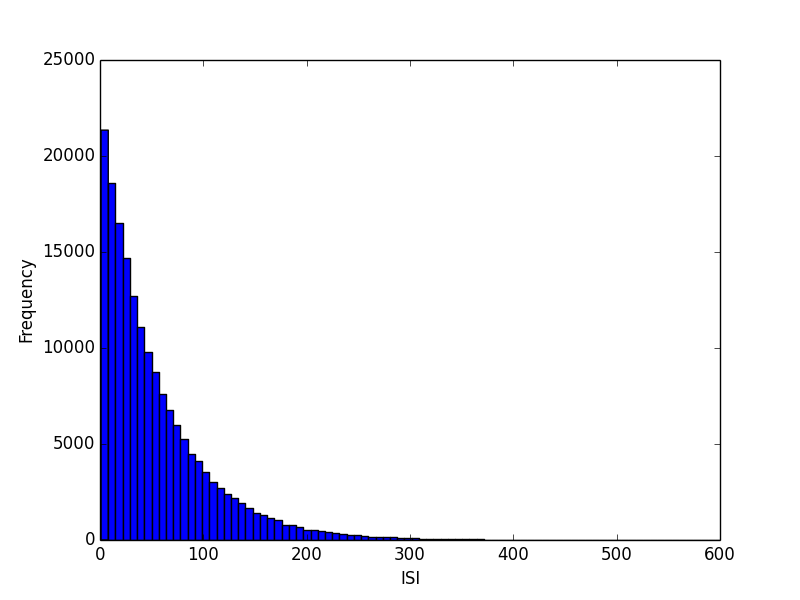
\includegraphics[scale=0.3]{EXP1_isiPOI.png}
				    \label{fig14:b}
			    }
			    \caption{
			        Distribution of ISI from the activity of $1000$ cells 
			        sampled from \emph{(a)} the TM, and \emph{(b)} a Poisson spiking model.
			        The activity from both models is practically indistinguishable.
			    }
			    \label{fig14}
		    \end{figure}
            
            In order to study how frequent binary patterns occur in the TM, 
            and how does this frequency compares to
            the random Poisson model we sampled $N = 10$ cells from both models by considering their complete spike
            history throughout the simulation.
            Then, following Ref.~\cite{schneidman2006weak}, we generated all $2^{N}$ binary patterns possible, and
            estimated the probability of observing each of them in the samples obtained from the TM and the random
            model.
            We repeated this process for $100$ trials.

            In Fig.~\ref{fig15} we show the probability of observing binary words of length $N = 10$
            in the TM in the random and high-order scenarios compared to the probability of observing 
            them in the Poisson spiking model.
            Each blue dot represents a binary word, e.g. $[1 0 1 1 0 0 1 1 0 1]$, from the total 
            $2^{10} = 1,024$ possible words.
            The solid black line represents the identity function; a point lying in this line represent
            binary words that occur as frequently as predicted, whereas points lying below (above) the line
            denote binary words that occurred more (less) frequent than predicted by the random model.
            
            In Fig.~\ref{fig15:a} dots close to the right top corner, which happen to occur very frequently
            and with the same probability in the TM and the Poisson model, correspond to binary patterns
            with only one bit ``on''.
            Similarly, the dots in the middle of the figure, which happen to occur more frequent in
            the TM than predicted by the Poisson model, correspond to binary patterns with only two
            bits ``on''.
            The dots close to the upper left corner correspond to binary patterns with $3$ or more
            bits ``on".
            Here, there are patterns that occur more frequently than predicted by the random model,
            as well as patterns that occur less often than predicted by chance.
            Likewise, in Fig.~\ref{fig15:b} dots in the upper-right corner correspond to binary patterns
            with only one bit ``on'', whereas the dots in the bottom-left corner correspond to patterns
            with more than one bit ``on".
            
            Does the TM behave like a Poisson spiking model?
            We began this section presenting results that suggest that the TM behaves like a Poisson spiking
            model during the early stages of learning for the random and high-order scenarios.
            We showed how the spiking activity of the TM resembles that of a Poisson spiking model 
            (see Figs.~\ref{fig13} and \ref{fig14}).
            However, when it comes to considering population of neurons representing binary patterns, 
            and comparing their occurrence to a random model, the situation looks different.
            If the TM behaved like a Poisson spiking model, then when looking at particular
            patterns of $N$ number of bits, we would expect them to occur as frequent as 
            predicted by the model.
            However, this is not the case, and some binary patterns occur more often than
            predicted, while others are in the opposite situation.
            This suggests that binary patterns do not occur in a random fashion, and that
            in fact the activation of cells in the TM is not completely independent from
            one another although the distribution of pairwise correlations points to the
            opposite idea.
            
            The activation of cell populations (in this case of size $N = 10$) carries meaningful
            information for the whole network.
            In summary, we observed that the probability of observing particular binary patterns 
            in the TM is larger than predicted from the random model. 
            This implies, as in the study by Schneidman et al., and 
            others~\cite{schneidman2006weak,koster2014modeling,berkes2011spontaneous}, that although pairwise
            correlations are weak, the network exhibits strong correlated states in the form of synchronous
            activity of neurons that represent useful information to the population.

 		 %   \begin{figure}[t]
			 %   \centering
			 %   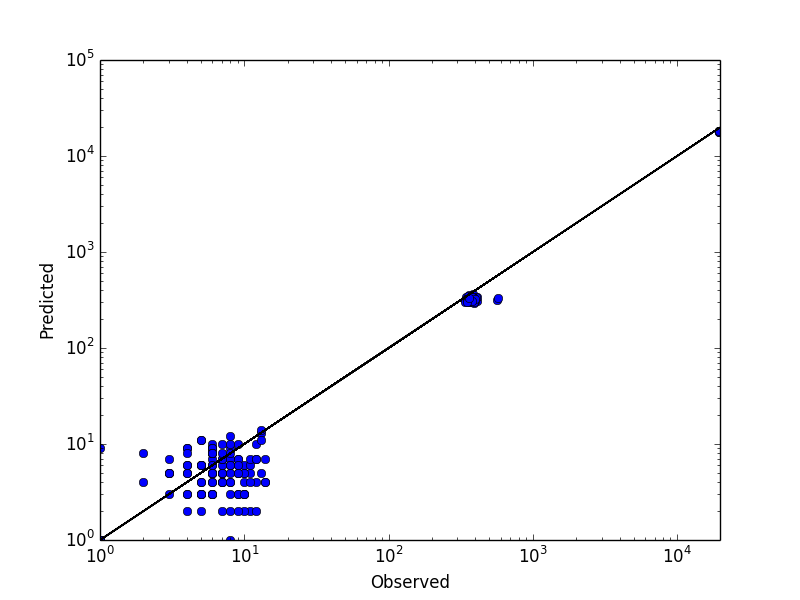
\includegraphics[scale=0.5]{EXP1_EladPlot.png}
			 %   \caption{
				%     Frequency of occurrence
				%     of binary patterns in the TM (\emph{observed}) vs. the frequency
				%     predicted by the random model (\emph{predicted}).
				%     Solid black line represents identity.
				%     (Read text.)
			 %   }
			 %   \label{fig15}
		  %  \end{figure}

		    \begin{figure}[t]
			    \centering
			    \subfloat[Random]{%
				    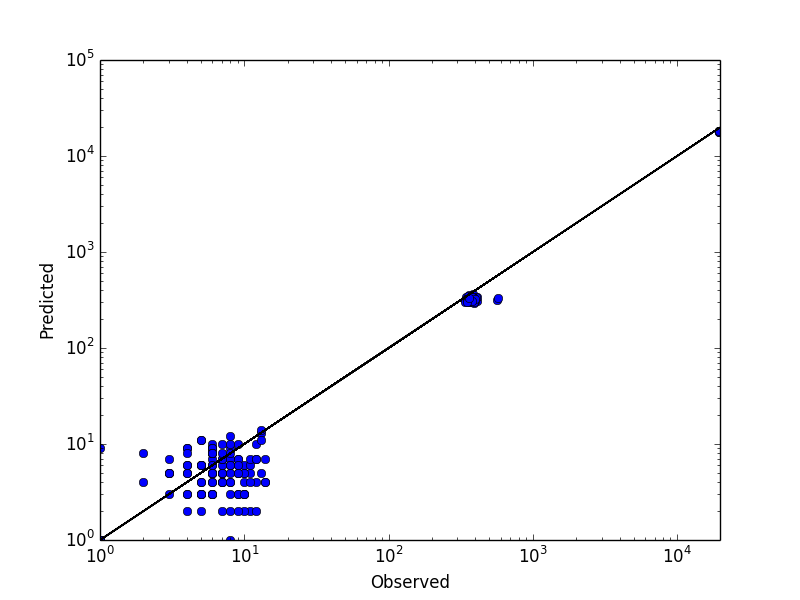
\includegraphics[scale=0.3]{EXP1_EladPlot.png}
				    \label{fig15:a}
			    }
			    \subfloat[High-order]{%
				    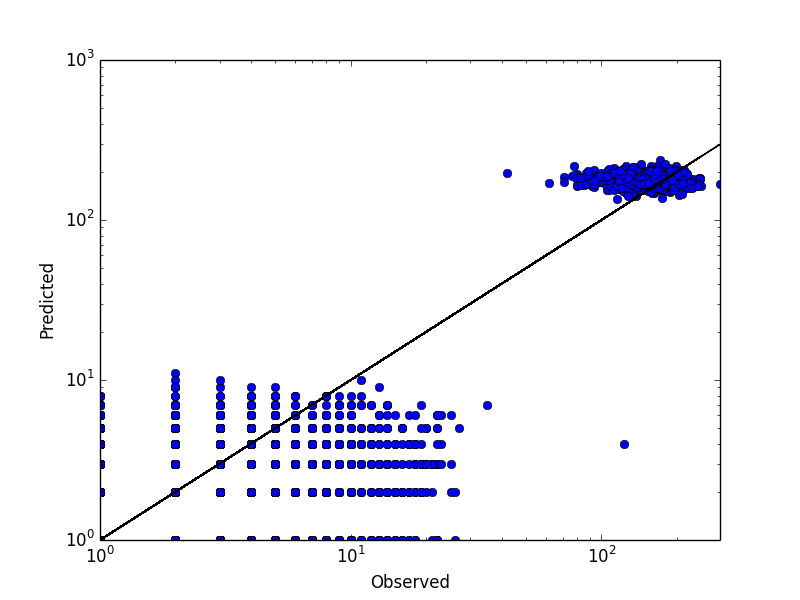
\includegraphics[scale=0.3]{EXP2_EladPlot.png}
				    \label{fig15:b}
			    }
			    \caption{
				    Frequency of occurrence
				    of binary patterns in the TM (\emph{observed}) for the random and
				    high-order scenarios vs. the frequency
				    predicted by the random model (\emph{predicted}).
				    Solid black line represents identity.
				    (Read text.)
			    }
			    \label{fig15}
		    \end{figure}
		    
		    
		    These observations were obtained in the random and high-order scenarios when the TM
		    was presented with the dataset only once, that is, the number of epochs was one.
		    What happens when we increase the number of training periods in the TM?
		    As we increase the learning periods in the TM, the activity of the network resembles
		    that of a Poisson spiking model even less.
		    For instance, the distribution of waiting times (ISI) exhibits a long right-tail,
		    which implies the presence of many cells with very short inter-spike intervals (high firing rate)
		    coexisting with cells whose inter-spike intervals are very large (low firing rate).
		    A Poisson spiking model cannot account for these observations. 
		    
		    Figure \ref{fig16} shows the ISI distribution from the activity of a sampled group of
		    cells in the TM when it was exposed to $5$ training periods in the random scenario.
		    It can be seen that there is a large number of cells with very short waiting times, that
		    is, cells that are firing very often. Then, the distribution decays abruptly leaving
		    a slowly-decaying right tail, which implies the presence of few cells whose waiting times are very large
		    but it is not negligible.
		    
 		    \begin{figure}[t]
			    \centering
			    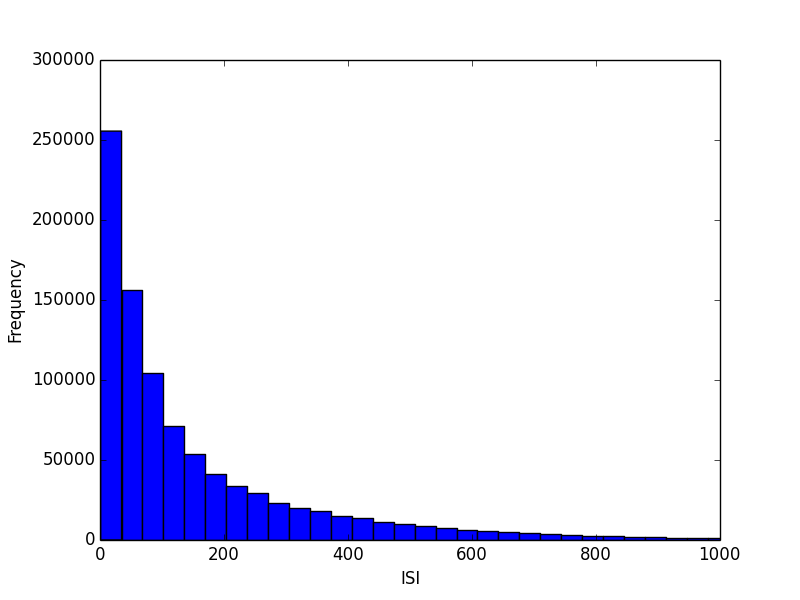
\includegraphics[scale=0.5]{EXP1_isiTM_epochsTM15.png}
			    \caption{
			        ISI distribution of the TM for the random scenario. 
			        Here, we exposed the TM with $15$ training periods.
			        Unlike Fig.~\ref{fig14:a}, the distribution exhibits an abrupt
			        decay and a slow decaying right tail.
			    }
			    \label{fig16}
		    \end{figure}	
		    
		    We measured the \emph{coefficient of variation}, which characterizes the variability in the inter-spike
		    intervals~\cite{heeger2000poisson}.
		    This coefficient is given by:
		    \begin{equation}
		        C_{V}= \frac{\sigma_{isi}}{\langle isi\rangle}
		    \end{equation}
		    
		    \noindent where $\langle isi\rangle$ refers to the mean of the inter-spike interval, whereas
		    $\sigma_{isi}$ refers to its standard deviation.
		    It is known that a coefficient of variation of unity is a property of a Poisson 
		    process~\cite{heeger2000poisson}.
		    When measuring this coefficient on the ISI distribution of the TM after $5$ periods of 
		    training, we obtained $C_{V} > 1$, whereas when there is no training periods
		    (epochs $ = 0$) the estimation of the coefficient yielded $C_{V} \approx 1$.
		    
		    This particular shape of the ISI distribution was observed in the other scenarios, namely,
		    high-order, NYC taxi dataset, and noisy sinusoid dataset.
		    In these cases, the ISI distribution exhibits a slowly-decaying right tail even in the absence
		    of training periods.
		    Figure \ref{fig17} shows the ISI distribution of the remaining scenarios (high-order, NYC taxi dataset
		    and the noisy sinusoid dataset).
		    All of these cases show a slowly-decaying right tail, which marks a divergence from the random Poisson
		    spiking model.
		    
		    \begin{figure}[t]
			    \centering
			    \subfloat[High-order]{%
				    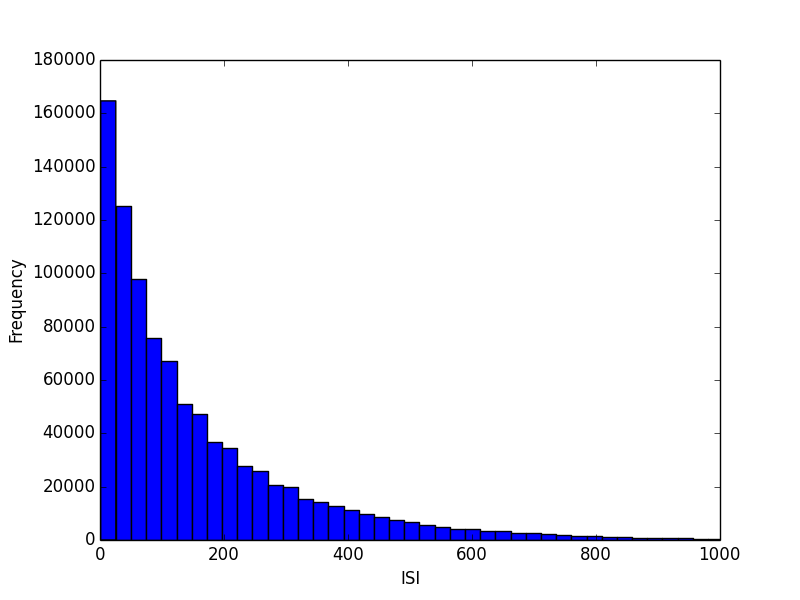
\includegraphics[scale=0.3]{EXP2_isiTM.png}
				    \label{fig17:a}
			    }
			    \subfloat[NYC taxi dataset]{%
				    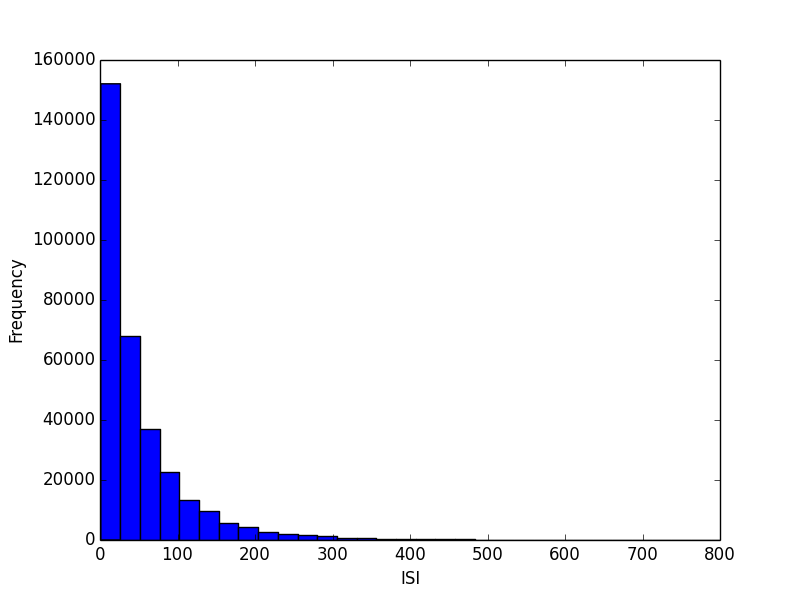
\includegraphics[scale=0.3]{EXP3_isiTM.png}
				    \label{fig17:b}
			    }\\
			    \subfloat[Noisy sinusoid]{%
				    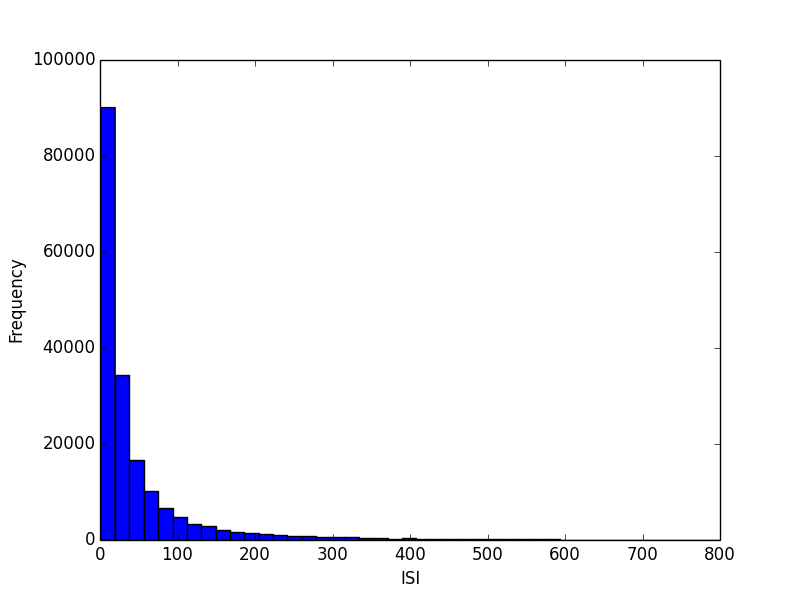
\includegraphics[scale=0.3]{EXP4_isiTM.png}
				    \label{fig17:c}
			    }			    
			    \caption{
			        ISI distributions for the three remaining scenarios considered in our experiments.
			        For the high-order scenario (\emph{a}), training periods were greater than one.
			        In all these cases, the distribution exhibits a slowly-decaying right tail.
			    }
			    \label{fig17}
		    \end{figure}		    
		    
            Thus, in summary when it comes to the shape of the ISI distribution we observe two types of behaviour:
            \begin{itemize}
                \item\emph{Exponential.} The distribution resembles an exponential distribution, which is known to
                reflect the presence of a Poisson spiking model~\cite{heeger2000poisson}. This behaviour is observed
                in the random and high-order scenarios in the absence of training periods, which means that 
                the TM observes every sequence only once.
                \item\emph{Long tail.} The distribution looks like a power-law distribution with a slow-decaying
                right tail. This implies the existence of many cells whose firing rate is large coexisting with
                a few cells with low firing rate, and whose existence is non-negligible.
                This behaviour was observed in the random and high-order scenarios when the TM is exposed to training periods
                (epochs $> 1$), as well as all other scenarios even in the absence of training periods for the TM.
            \end{itemize}
            
            What is the origin of these two different behaviours of the ISI distribution?
            We hypothesize that the origin of this behaviour is related to the amount of novelty and
            familiarity that the TM has for the incoming input.
            A sequence of SDRs is fed to the TM.
            If the SDR is novel to the TM, then a set of columns burst.
            This increases the spiking activity in the TM, making it denser.
            This in turn, results in activity that can be approximated by a Poisson spiking model
            with certain accuracy.
            However, as the TM is presented with familiar input, complete columns stop bursting
            and the activity becomes sparser with few cells firing constantly and a majority of cells
            firing sporadically.
            
            Figure \ref{fig18} shows the distribution of spike counts from samples of $1000$ cells
            in all scenarios considered and no training periods.
            The random and high-order cases yield a more symmetrical distribution than the other cases. 
            Moreover, these are the only case that can be related to a Poisson spiking model.
            The other distributions exhibit a tendency to develop a right tail which implies the existence
            of a few cells that spike frequently.
            
		    \begin{figure}[t]
			    \centering
			    \subfloat[Random]{%
				    \includegraphics[scale=0.3]{EXP1_spikesHist_TM.png}
				    \label{fig18:a}
			    }
			    \subfloat[High-order]{%
				    \includegraphics[scale=0.3]{EXP2_spikesHist.png}
				    \label{fig18:b}
			    }\\
			    \subfloat[NYC taxi dataset]{%
				    \includegraphics[scale=0.3]{EXP3_spikesHist.png}
				    \label{fig18:c}
			    }
			    \subfloat[Noisy sinusoid]{%
				    \includegraphics[scale=0.3]{EXP4_spikesHist.png}
				    \label{fig18:d}
			    }			    
			    \caption{
			        Distribution of spike counts from the TM for all different scenarios and no training periods.
			    }
			    \label{fig18}
		    \end{figure}		    
            
            As mentioned above, when the TM receives familiar input, instead of bursting, all cells within a column will
            remain silent but one.
            A familiar input does not refer only to the same SDR occurring in different times during an experiment, 
            but also to SDRs that have high overlap among each other.
            
            The cumulative effect of column bursting increases the activity within the network resulting in an exponential
            shape of the ISI distribution, and its subsequent approximation to a Poisson spiking model.
            On the opposite, when columns stop bursting as a result of familiar input to the TM, the activity
            becomes sparser which results in the long-tail distribution of inter-spike intervals.
            
            Power-law distributions of inter-spike intervals have been related to the conditional maximization
            of firing-rate entropy (CMFE)~\cite{tsubo2012power}.
            This hypothesis states that \emph{in vivo} cortical neurons try to maximize the amount of
            information represented by their spike trains while keeping metabolic costs and 
            uncertainty on output spike trains at minimum.
            It has been shown that a consequence of neurons operating under such constraints is the
            emergence of long and slow-decaying tails in ISI distributions~\cite{tsubo2012power}.
            
            Although a more rigorous examination is still underway,
            the ISI distributions in our experiments resemble a power-law distribution with slowly-decaying
            right tails that could relate the activity of the TM with large training periods to the CMFE hypothesis. 
            This will be a direction of future research.
            
		    
        \subsection{Neural activity becomes sparse as learning increases}
        
		    The particular shape of the ISI distribution (Fig.~\ref{fig16}) is correlated with
		    the activity within the TM becoming sparser.
            In other words, as the training epoch increases the activity in the TM becomes
            sparser.
            The phenomenon of sparse neural activity correlated with learning has been reported 
            in experimental settings elsewhere~\cite{averbeck2006neural,cohen2011measuring}.
            
            In Fig.~\ref{fig19} we present the evolution of the spike count for all cases considered.
            In most cases the trace exhibits a decreasing trend that implies that the activity is
            decreasing within the network as the TM learns from its input.
            % For the purpose of analyzing this trend, we increased the learning periods of the TM in
            % the NYC taxi and noisy sinusoid scenarios.
            % Here, we ran $3$ training periods, which means that we fed the whole dataset $3$ times
            % without resetting the TM after each presentation for the purpose of keeping track of the
            % spike count trace for longer periods of time.
            In the NYC taxi and noisy sinusoid datasets we observe that although the trace is non-monotic, 
            it exhibits a decreasing trend.

		    \begin{figure}[t]
			    \centering
			    \subfloat[Random]{%
				    \includegraphics[scale=0.3]{EXP1_numSpikesTrace.png}
				    \label{fig19:a}
			    }
			    \subfloat[High-order]{%
				    \includegraphics[scale=0.3]{EXP2_numSpikesTrace.png}
				    \label{fig19:b}
			    }\\			    
			    \subfloat[NYC taxi]{%
				    \includegraphics[scale=0.3]{EXP3_numSpikesTrace.png}
				    \label{fig19:c}
			    }
			    \subfloat[Noisy sinusoid]{%
				    \includegraphics[scale=0.3]{EXP4_numSpikesTrace.png}
				    \label{fig19:d}
			    }
			    \caption{
			        Evolution of spike count in all scenearios considered.
			        In most cases the trace exhibits a decreasing trend implying that the
			        activity within the network is becoming sparser.
			    }
			    \label{fig19}
		    \end{figure}		    
            
            In Fig.~\ref{fig20} we present some examples of raster plots for two scenarios: random and high-order, at
            two stages of the learning process.
            Activity within the network is dense at the early stages of learning, but it becomes sparse as learning
            continues.

		    \begin{figure}[t]
			    \centering
			    \subfloat[Random scenario: early stages]{%
				    \includegraphics[scale=0.3]{EXP1_rasterTM_before.png}
				    \label{fig20:a}
			    }
			    \subfloat[Random scenario: later stages]{%
				    \includegraphics[scale=0.3]{EXP1_rasterTM_after.png}
				    \label{fig20:b}
			    }\\			    
			    \subfloat[High-order scenario: early stages]{%
				    \includegraphics[scale=0.3]{EXP2_rasterTM_before.png}
				    \label{fig20:c}
			    }
			    \subfloat[High-order scenario: later stages]{%
				    \includegraphics[scale=0.3]{EXP2_rasterTM_after.png}
				    \label{fig20:d}
			    }
			    \caption{
			        Raster plots of two scenarios: \emph{(a)} and \emph{(b)} Random, 
			        and \emph{(c)} and \emph{(d)} High-order.
			        The activity in the early stages of learning is denser (\emph{a} and \emph{c}) than
			        in its later stages (\emph{b} and \emph{d}).
			    }
			    \label{fig20}
		    \end{figure}		    

            In Fig.~\ref{fig21} we present examples of raster plots for the other two scenarios: 
            NYC taxi and noisy sinusoid datasets.
            In such plots it is less evident that the activity within the network is becoming sparser
            as learning continues.
            However a look at Fig.~\ref{fig22} gives a clearer idea of how sparsity evolves during
            learning.
            
            
		    \begin{figure}[t]
			    \centering
			    \subfloat[NYC taxi dataset: early stages]{%
				    \includegraphics[scale=0.3]{EXP3_rasterTM_before.png}
				    \label{fig21:a}
			    }
			    \subfloat[NYC taxi dataset: later stages]{%
				    \includegraphics[scale=0.3]{EXP3_rasterTM_after.png}
				    \label{fig21:b}
			    }\\			    
			    \subfloat[Noisy sinusoid scenario: early stages]{%
				    \includegraphics[scale=0.3]{EXP4_rasterTM_before.png}
				    \label{fig21:c}
			    }
			    \subfloat[Noisy sinusoid scenario: later stages]{%
				    \includegraphics[scale=0.3]{EXP4_rasterTM_after.png}
				    \label{fig21:d}
			    }
			    \caption{
			        Raster plots of two scenarios: \emph{(a)} and \emph{(b)} NYC taxi dataset, 
			        and \emph{(c)} and \emph{(d)} noisy sinusoid.
			        Activity within the network is denser in the early stages of training than
			        in later stages. However, unlike Fig.~\ref{fig20}, the decrease in activity
			        is not too pronounced.
			    }
			    \label{fig21}
		    \end{figure}
		    
		    Figure \ref{fig22} shows the sparsity trace of all scenarios considered.
		    The $y$ axis of this plot represents the percentage of cells active in function
		    of time. From a total of $16,384$ cells in the network, $2\%$ activity corresponds
		    to roughly $320$ cells, which correspond to $40$ columns bursting as a result of
		    novel input being presented to the TM.
		    In a situation in which the TM learns accurately its input, whenever the TM is
		    presented with a correctly predicted SDR only $40$ cells will become active,
		    this corresponds to roughly $0.2\%$ of cells active at a given time.
		    
		    In all cases considered the network converges to a sparse state of activity in
		    which only a few cells are active.
		    This behaviour is expected. As the TM learns from its input, less cells become
		    active up to a point in which only $40$ cells are active when there is perfect accuracy.
		    The shape and speed of the decrease of activity within the network depends on the
		    nature of the dataset.

		    \begin{figure}[t]
			    \centering
			    \subfloat[Random]{%
				    \includegraphics[scale=0.3]{EXP1_sparsityTrace.png}
				    \label{fig22:a}
			    }
			    \subfloat[High-order]{%
				    \includegraphics[scale=0.3]{EXP2_sparsityTrace.png}
				    \label{fig22:b}
			    }\\			    
			    \subfloat[NYC taxi dataset]{%
				    \includegraphics[scale=0.3]{EXP3_sparsityTrace.png}
				    \label{fig22:c}
			    }
			    \subfloat[Noisy sinusoid]{%
				    \includegraphics[scale=0.3]{EXP4_sparsityTrace.png}
				    \label{fig22:d}
			    }
			    \caption{
			        Sparsity trace for all scenarios considered.
			        In all cases considered activity within the network tends
			        to become sparser. 
			        The speed in which this occurs depends on the nature
			        of the dataset.
			    }
			    \label{fig22}
		    \end{figure}
        
        \subsection{Learning increases the amount of negative correlations}
        
            Next we investigated on the effect of learning over the structure of pairwise
            neural correlations.
            We expected the amount of negative correlations increase as the
            TM learns the input.
            The reason behind this hypothesis is the following:
            novel input causes columns within the TM to burst, this leads to
            positively correlated activity of the cells within the bursting columns.
            As the TM learns the sequence, cells within columns stop bursting and
            on the contrary, we would observe only one cell per column becoming active.
            This leads to negative correlations among cells within the same column.
            This in consequence would lead to an increase in the number of negative
            correlations, once the TM learns its input better.
            
            For scenarios such as the random and high-order cases, we were required to
            inspect the number negative correlations while the TM learns from the input,
            whereas for the NYC taxi and noisy sinusoid scenarios we required to
            assess the amount of negative correlations also as an effect of learning
            by the SP.
            
            We report that negative pairwise correlations increase when increasing the
            training periods of the TM in all cases considered.
            Figure \ref{fig23} shows the trace of the number of negative pairwise
            correlations.
            Here, the TM was learning while data was being presented to it.
            The amount of negative neural correlations increase with time as a result
            of training.

		    \begin{figure}[t]
			    \centering
			    \subfloat[Random]{%
				    \includegraphics[scale=0.3]{EXP1_negPCCTrace.png}
				    \label{fig23:a}
			    }
			    \subfloat[High-order]{%
				    \includegraphics[scale=0.3]{EXP2_negPCCTrace.png}
				    \label{fig23:b}
			    }\\
			    \subfloat[NYC taxi dataset]{%
				    \includegraphics[scale=0.3]{EXP3_negPCCTrace_TM.png}
				    \label{fig23:c}
			    }
			    \subfloat[Noisy sinusoid]{%
				    \includegraphics[scale=0.3]{EXP4_negPCCTrace_TM.png}
				    \label{fig23:d}
			    }
			    \caption{
			        Trace of amount of pairwise negative correlations all experiments.
			        The number of negative correlations increases with training until 
			        saturation (\emph{a} and \emph{b}).			        
			    }
			    \label{fig23}
		    \end{figure}
		    		    
		    Moreover, we observed that the training periods in the SP have
		    an effect on the number of negative pairwise correlations in the TM.
		    Here, we varied the number of training items for the SP.
		    This not only has an impact on the amount of negative correlations
		    emerging in the TM, but also in the frequency in which columns become
		    active.
		    As mentioned above, we refer to this as \emph{column usage} and 
		    we showed two examples of these distributions in Figs.~\ref{fig8} and \ref{fig9}.
		    These plots present the distribution of the number of times that a column
		    has been active during simulation time.
		    A tail in this distribution implies the existence of columns that are
		    active very frequently.
		    
		    In Fig.~\ref{fig24} we present the trace of the number of negative
		    pairwise correlations in function of the training items in the SP.
		    Here we fixed the number of training periods in the SP but varied the number
		    of items in the training set of the SP.
		    In the case of the NYC taxi dataset (Fig.~\ref{fig24:a}) the number of
		    negative pairwise correlations exhibit an increasing trend, whereas
		    for the noisy sinusoid dataset (Fig.~\ref{fig24:b}) the trend is not clear.
		    
		    In sum, we conclude that the amount of negative pairwise correlations
		    increases with training in the experiments considered.
		    However we were not able to verify that this phenomenon is clearer when sampling
		    from cells within same columns as the process of choosing cells might be
		    choosing cells from columns that are never active, or that become active sparsely
		    as a result of the particular input being presented to the TM.

		    \begin{figure}[t]
			    \centering
			    \subfloat[NYC taxi dataset]{%
				    \includegraphics[scale=0.3]{EXP3_negPCCTrace_SP.png}
				    \label{fig24:a}
			    }
			    \subfloat[Noisy sinusoid]{%
				    \includegraphics[scale=0.3]{EXP4_negPCCTrace_SP.png}
				    \label{fig24:b}
			    }
			    \caption{
			        Amount of negative pairwise correlations in function of training items
			        in the SP for the NYC taxi (\emph{a}) and noisy sinusoid (\emph{b}) datasets.
			    }
			    \label{fig24}
		    \end{figure}
		    
    \section{Conclusions}
        
        We have shown that for the random and high-order scenarios, the TM behaves almost like a 
        Poisson spiking model in the absence of training. However, when measuring the rate in which
        binary patterns occur we observe that its behaviour differs from that of a random spiking model,
        and some patterns occur with more or less frequency than predicted.
        This analysis is a proxy for studying higher order correlations, that is, correlations
        that go beyond simple neuron pairs.
        
        However, in the presence of learning (epochs $> 1$) the TM not longer behaves like a Poisson
        spiking model. This can be observed both in the shape of the distribution of inter-spike intervals
        as well as in the coefficient of variation, which becomes larger than unity with longer training
        periods.
        This observation is valid for the random and high-order scenarios when training periods are larger than
        unity, as well as for the NYC taxi and noisy sinusoid scenarios.
        In the last two cases the observation was valid even when the TM was exposed to the data only once.
        We believe that this is due to the nature of the data, which exhibits large overlapping scores, 
        implying that some SDRs might resemble each other. 
        This in consequence is interpreted by the TM as already-seen input.
        We showed how the distribution of the inter-spike intervals exhibits a slow-decaying right tail
        which has several implications on neural computation.
        Nevertheless, such implications remain to be explored in the current model.
        
        We have shown as well that in all scenarios considered pairwise correlations are weak, and learning
        has the effect of reducing the amount of positive correlations.
        Moreover, we have shown how learning increases the amount of anti-correlated activity captured by the
        presence of negative correlations.
        This phenomenon is also related to the training parameters in the spatial-pooler for cases in which
        we use real numbers as input to the TM.
        
        Thus, based in our observations we present the following predictions which might be testable in 
        an experimental setting involving learning in neocortical tissue:
        \begin{itemize}
            \item Sequence learning in the neocortex has the effect of weakening pairwise neural correlations.
            \item Learning might increase the amount of negative correlations. This observation will
            be related to the nature of the stimuli being fed to the network.
            Random input could be thought of artificial stimuli, whereas periodic input could be thought of
            natural stimuli.
            \item As well, this results in sparse activity within a neural network. This has also been
            hypothesized elsewhere in experimental neuroscience.            
            \item The distribution of inter-spike intervals will exhibit a slowly-decaying right tail
            that will resemble a power-law distribution as a result of learning.
        \end{itemize}
        
        Further direction of work includes fitting a model to the TM at later stages of learning in order to
        repeat the Schneidman analysis comprising binary words and comparing their rate of occurrence between
        random model and TM. As well, further work includes the design of experiments that are more akin
        to computational neuroscience such as the presentation of bars to the TM.
        Lastly, we should as well investigate more about the implications of observing heavy-tailed distributions
        of inter-spike intervals in theoretical and experimental neuroscience.
    
    \bibliographystyle{plain}
    \bibliography{biblio}
    
\end{document}